% !TeX program = xelatex

\documentclass[12pt,a4paper]{article}

\usepackage[UTF8,scheme=chinese]{ctex}
\usepackage{xeCJK}
\usepackage{url}
\usepackage{hyperref}
\usepackage{graphicx}
\usepackage{geometry}
\usepackage{setspace}
\usepackage{amsmath}
\usepackage{amsfonts}
\usepackage{amssymb}
\usepackage{cite}
\usepackage{fontspec}
\usepackage{multirow}

\setmainfont{Times New Roman}

\setCJKmainfont{標楷體}

\newCJKfontfamily\kaiFakeBold[FakeBold=2]{標楷體}

\makeatletter
\renewcommand\bfseries{
  \kaiFakeBold
  \fontseries\bfdefault\selectfont
}
\makeatother

\ctexset{
    contentsname={目錄},
    listfigurename={圖目錄},
    listtablename={表目錄},
    figurename={圖},
    tablename={表},
    abstractname={摘要},
    indexname={索引},
    appendixname={附錄},
    bibname={參考文獻}
}

% 基本套件


% 頁面設定
\geometry{
    left=3cm,
    right=2cm,
    top=2.5cm,
    bottom=2.5cm
}

% 行距設定
\onehalfspacing

\begin{document}
\begin{titlepage}

	\centering
	\vspace*{2cm}
	
	{\Large 國立臺灣海洋大學\\[0.5cm]資訊工程系專題報告 \par}
	
	\vspace*{1cm}
	{\Huge 智慧化AI船舶群集搜救規劃系統 \par}
	
	\vfill
	
	{\Large 指導教授:鄭錫齊\ 教授 \par}
	\vspace*{1cm}
	\begin{tabular}{lll}
	學號 & 姓名 & E-mail \\
	\hline
	01157001 & 黃品翰 & hanshuangfs@gmail.com \\
	01157026 & 馮宥崴 & wallacef930814@gmail.com \\
	01157045 & 唐予安 & anthonyaa0423@gmail.com \\
	01157152 & 巫侑霖 & gray930522@gmail.com
	\end{tabular}

	\vspace*{1cm}
	{\Large 中華民國\ 114 年\ 9 月\ 21 日 \par}

\end{titlepage}

% 摘要
\vspace*{0.3\textheight}
\begin{abstract}
本研究提出一套「智慧化AI船舶群集搜救規劃系統」,旨在改善海上的搜救方式。傳統的搜救常常面臨海象險惡、作業風險高及搜尋範圍廣闊等挑戰,很容易錯過黃金救援時間,且存在高危險性。本研究希望透過無人船群集的系統化應用,透過現代 AI 技術進行更有效率的搜尋,以降低搜救人員傷亡風險,同時提升大範圍搜尋的效率,解決現有搜救作業的困難。
\par
為因應上述挑戰,本系統以無人船群集協作為核心,透過強化學習演算法規劃搜救路徑,並可根據海流、風向等環境因素即時調整搜尋方向。由於缺乏實體船舶作為驗證平台,本研究採用 Unity 模擬環境進行系統建構與實驗,並針對單人與多人落水情境進行測試,驗證其可行性。
\par
實驗結果顯示,本系統在單一落水搜救情境下達到 82\%  的搜尋成功率,相較於傳統人工搜尋僅約 50\%  的成功率有顯著提升;在多人落水的情況下,系統能搜尋到 78\%  的落水人員。此外,針對因風向影響的落水人員移動,本系統的預測準確率達 81\%。
\par
本研究的貢獻在於證實無人船群集應用於海上搜救的潛力,能有效降低人力風險並縮短救援時間。未來若能進一步導入真實海域測試,並結合感應器精度、通訊穩定性及實際惡劣天候下的作業考量,將更加貼近實際應用的需求,並提升系統的實用價值。

\end{abstract}

\centerline{\textbf{關鍵詞:} 船舶群集、搜救系統、深度強化學習、多代理人系統、海洋模擬}

\newpage

% 目錄
\tableofcontents

\vspace*{2cm}

% 組員貢獻表格
\section*{組員貢獻}
\addcontentsline{toc}{section}{組員貢獻}

\begin{table}[h]
\centering
\begin{tabular}{|c|p{8cm}|c|}
\hline
\textbf{組員姓名} & \textbf{主要貢獻內容} & \textbf{貢獻比例} \\
\hline
黃品翰 & 海洋環境架設、進行訓練、訓練環境架設、模型配置設計與調教、具象化實驗結果、撰寫相關文件、整理實驗結果 & 25\% \\
\hline
唐予安 & 撰寫相關文件、進行訓練、獎勵函數設計、訓練流程規劃、整理相關文獻 & 25\% \\
\hline
馮宥崴 & 調查海上搜救方法、整理相關文獻、海洋環境架設、搜救實驗規劃、撰寫相關文件、整理實驗結果 & 25\% \\
\hline
巫侑霖 & 系統架構規劃、核心模組程式碼實作、查閱技術文件、模型配置設計與調教、進行模型訓練、進行實驗& 25\% \\
\hline
\end{tabular}
\end{table}

\newpage

% 正文開始
\section{緒論}

\subsection{研究背景與動機}
海洋覆蓋地球表面超過七成,是全球貿易、資源開發與休閒活動的核心場域。然而,隨著海上交通與作業日益頻繁,船舶事故、惡劣氣候與人員落水的風險持續上升。一旦發生事故,搜救(Search and Rescue, SAR)行動成為攸關人命的即時挑戰,其中「救援時間」決定了受困者的生存率\cite{NOAA}。

傳統搜救模式仰賴人員經驗與指揮調度,在大範圍海域與高風險環境下常受限於人力與效率。隨著人工智慧(AI)、自主系統(Autonomous Systems)與高擬真模擬技術的成熟,發展基於智慧化與自主化的搜救系統已成為突破現有困境的契機。自主船舶群集可藉由耐航性、即時協作與精確導航,提升搜救任務的速度與覆蓋範圍,進而增加受困人員的獲救機率\cite{GroupMobile}。本研究即在此背景下展開。

\subsection{問題陳述}
雖然自主船舶與強化學習的應用具有強大的潛力,能夠在大多任務中提升效率與反應速度,但在搜救場景中仍面臨多重挑戰\cite{KilicChallenge}\cite{KilicRL}\cite{NOAA}:

\begin{enumerate}
\item \textbf{搜索效率不足}:傳統搜索在大範圍海域下難以兼顧效率與覆蓋率。
\item \textbf{環境動態與不確定性}:風浪與洋流使船隻航行與感測受干擾,增加搜尋難度\cite{IAMSAR2008}。
\item \textbf{群集協同複雜性}:多艘船隻需避免搜尋範圍重疊、確保安全並即時共享資訊\cite{IAMSAR2008}。
\item \textbf{時間壓力與決策挑戰}:有限時間內需快速分配資源並做出最佳判斷,錯誤可能導致錯失救援時機。
\end{enumerate}

因此,有必要建構一個智慧化模擬系統,以驗證各種策略並最佳化搜救行動。

\subsection{研究目的}
本研究的目標在於建立一個「智慧化AI船舶群集搜救規劃系統」,具體目的如下:

\begin{itemize}
\item \textbf{建立高擬真模擬環境}:以 Unity 與 Crest 套件模擬真實海象與物理效果,作為測試平台。
\item \textbf{開發自主搜救代理人}:利用深度強化學習演算法,訓練船舶於動態環境中進行自主導航與避障。
\item \textbf{設計群集協同策略}:透過分區搜尋與任務分配,提升多船協同效率,避免重複與衝突。
\item \textbf{效能評估與驗證}:以模擬實驗檢驗系統在搜尋成功率、平均搜救時間與協同效率上的成效。
\end{itemize}

\subsection{相關使用技術介紹}

本系統整合以下技術,以實現智慧化船舶群集搜救模擬與訓練:

\begin{itemize}
	\item \textbf{Soft Actor-Critic (SAC)}:基於最大熵強化學習的演算法,透過 actor-critic 架構、雙 Q 網路與熵正則項,同時追求回報最大化與策略多樣性,提供穩定且高效的策略學習 \cite{Atari}\cite{SAC}。
	\item \textbf{Unity3D}:跨平台 3D 開發引擎,支援物理模擬、場景可視化與高自由度控制,適合構建模擬環境。
	\item \textbf{ML-Agents}:將 Unity 環境轉化為代理人訓練場域,支援強化學習、模仿學習與自我對弈,訓練完成後可匯出模型直接部署\cite{MLAgentRepo}。
	 \item \textbf{Crest 海洋套件}:提供高品質水面渲染與波浪模擬,支援物理互動與光影效果,增強船舶模擬的真實感與環境互動性\cite{CrestIntro}。
\end{itemize}

\subsection{實驗方法與結果}
本研究在 Unity 與 Crest 海洋物理引擎所建構的模擬環境中,使用 SAC 深度強化學習演算法訓練自主船舶,以具備導航與避障能力。雖然整體系統設計為多代理架構,但為降低訓練複雜度與收斂時間,本研究採用單代理訓練,並利用「殭屍船」模擬多代理互動,以確保船舶能在動態環境中學習穩定航行與避障策略。

完成訓練後,系統進一步被應用於兩種搜救情境:  
\begin{itemize}
    \item \textbf{單一落水點快速救援}:模擬單人落水的情況,船隊需在有限時間內完成定位。共進行 359 次測試,成功率達 82\%,並且落水人員位置範圍預測正確率達 81\%。  
    \item \textbf{大範圍隨機搜尋任務}:模擬大規模事故中人員隨機散落的情境,共進行 109 次測試,模擬 1070 位落水人員,其中 831 人成功被定位與救援,成功率為 78\%。  
\end{itemize}

結果顯示,本系統在單人與多人落水情境下均能展現高成功率,並能因應海流與風向進行動態調整。相較於傳統人力搜尋約 50\% 的成功率,系統在覆蓋率與效率上皆有顯著提升,展現智慧化船舶群集於海上搜救任務的應用潛力。


\subsection{結果討論}
實驗結果顯示,本研究所建構的智慧化船舶群集搜救規劃系統能在動態海域環境中有效完成搜尋任務,得以在提高搜尋效率與覆蓋範圍的情況下,同時減少人力依賴並提升落海人員的獲救機率。  然而,本研究採用單代理訓練,尚未充分發揮多代理協作的潛在優勢。因此,未來研究可透過多代理強化學習、更多真實環境變因以及實地測試,進一步驗證系統效能並提升協作穩定性。



\newpage

\section{文獻回顧與討論}

\subsection{海上搜救相關研究}

\subsubsection{傳統海上搜救方法}
傳統的海上搜救方法在《IAMSAR 操作手冊》\cite{IAMSAR2008}\cite{Oways} 中有明確規範,常見的類型有:
\begin{itemize}
	\item \textbf{Expanding square search(擴展方形搜尋)}
	\begin{itemize}
		\item 適用於目標位置大致已知、中等範圍的搜尋。
		\item 搜尋點從基準點開始搜尋,每次往前一段距離後轉向 90 度,每次轉向航段都會逐漸加長。
		\item 需要準確的導航系統。
	\end{itemize}
	\item \textbf{Sector search(扇形搜尋)}
	\begin{itemize}
		\item 適用於目標位置明確、小範圍的搜尋。
		\item 搜尋方式由基準點為圓心,進行放射狀的搜尋。
		\item 最多只能由一艘船與一架飛機分別進行搜尋。
	\end{itemize}
	\item \textbf{Parallel sweep search(平行航線搜尋)}
	\begin{itemize}
		\item 適用於目標位置未知、大範圍的搜尋。
		\item 搜尋區域被劃分為多個子區域,由不同的船舶分工搜尋,每個子區域的搜尋航線互相平行,並與海流方向一致。
		\item 由於派出的單位較多,因此需要消耗大量的資源。
	\end{itemize}
\end{itemize}

\begin{figure}[h]
    \centering
    \begin{minipage}[t]{0.3\textwidth}
        \centering
        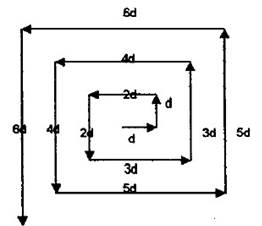
\includegraphics[width=\textwidth]{image/ExpandingSquareSearch.png}
        \caption{擴展方形搜尋}
    \end{minipage}%
    \hfill
    \begin{minipage}[t]{0.3\textwidth}
        \centering
        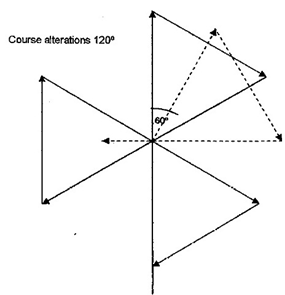
\includegraphics[width=\textwidth]{image/SectorSearch.png}
        \caption{扇形搜尋}
    \end{minipage}%
    \hfill
    \begin{minipage}[t]{0.3\textwidth}
        \centering
        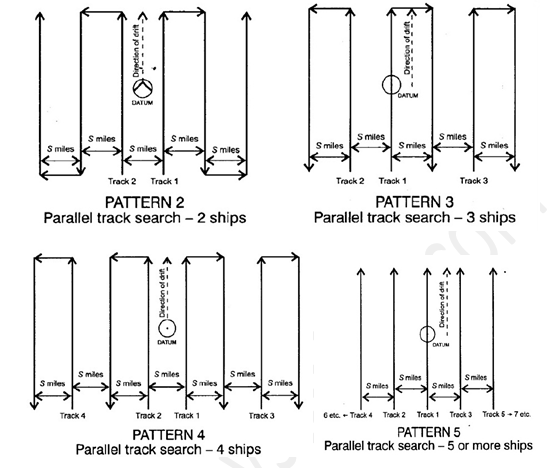
\includegraphics[width=\textwidth]{image/ParallelSweeepTrack.png}
        \caption{平行航線搜尋}
    \end{minipage}
\end{figure}


\subsubsection{傳統方法的限制與挑戰}
\begin{itemize}
  \item \textbf{安全風險}:傳統的搜救方式需要出動大量的人員與船舶,如在極端天候可能會造成額外的風險\cite{USCoastGuard}。
  \item \textbf{人力與資源消耗}:以平行航線為例,雖然能夠覆蓋較大的範圍,但同時也需要使用大量的船舶及人員,而搜救成本也隨之增加\cite{KilicChallenge}。
  \item \textbf{搜尋效率受限}:擴展正方形、扇形搜尋雖然成本相較為低廉,然而其搜尋範圍相對有限,並且在海流及海風的影響下,航線容易偏移,降低搜尋效率\cite{KilicChallenge}\cite{AiCoverage}。
  \item \textbf{時效性不足}:當目標位置未知且搜尋範圍過大,傳統的人工搜尋方法往往很難在黃金救援期間完成全面搜尋\cite{AiCoverage}。
\end{itemize}

\subsubsection{技術發展}
隨著科技進步,傳統搜救方式的限制逐漸被新技術所補足\cite{Ennong}:
\begin{itemize}
  \item \textbf{無人機}:具備高機動性,能在短時間內對大範圍的海域進行空中偵查。
  \item \textbf{自主船舶}:可執行長時間、低成本的搜尋,降低人員風險與油料消耗。使用群集作業可以補足平行航線搜尋的缺點,在維持大範圍的情況下同時減少搜尋成本。
  \item \textbf{混和搜救系統}:結合有人、無人船舶及無人機,形成「立體化」的搜尋網路。有人單位可以集中精力於高價值決策或特殊任務,無人單位負責長時間及大範圍的搜尋\cite{Survey}。
\end{itemize}

\subsection{自主船舶系統現代應用}
隨著無人化技術的推進,自主船舶在海洋產業中逐漸成熟並投入實際應用。主要集中在以下的面向\cite{autoboat}:
\begin{itemize}
  \item \textbf{任務自動化與導航精準度}:透過高精度 GPS 與自主導航演算法,使船舶能在無人操控下完成大範圍的搜尋與調查。
  \item \textbf{能源與續航力優化}:積極推動電力及太陽能的使用,用以滿足長時間海上作業的需求。
  \item \textbf{安全與可靠性}:增設船體健康監控、故障預警與各種感測器,以即時偵測船體外部環境進行自主避障。
  \item \textbf{應用多元化}:涵蓋貨運、離岸風電運維、海洋調查與急難救助等。
\end{itemize}

\paragraph{相關應用案例}
\begin{itemize}
  \item Yara Birkeland:全球首艘全電動無人貨櫃船,展現大型自主船舶的商轉潛力\cite{Yara}。
  \item 日本 MEGURI 2040 計畫:推動多艘無人渡輪與貨船運行,測試長距離自主航行能力\cite{Meguri}。
  \item 英國 Rolls-Royce、韓國現代重工:積極投入智慧船舶與自主航行技術\cite{Rolls}\cite{Hyundai}。
\end{itemize}

\subsection{深度強化學習於自主導航領域之研究}

\subsubsection{傳統演算法與限制}
在自主導航(Autonomous Navigation)領域中,傳統的路徑規劃方法如 A*、Dijkstra 與快速隨機樹(Rapidly-exploring Random Tree, RRT),一直是最為基礎且廣泛使用的演算法。然而,傳統演算法仍包含了許多限制\cite{PathPlanning}:
\begin{itemize}
  \item 缺乏即時適應性:當環境發生變化(如動態障礙物、移動目標)時,需重新規劃路徑,反應速度不足\cite{EnhancedPathPlanning}。
  \item 計算負擔大:在高維、複雜或大規模環境下,演算法的計算時間與記憶體需求急遽增加\cite{SimulationHeuristic}。
  \item 難以處理不確定性:傳統規劃多依賴完整或靜態的環境資訊\cite{EnhancedPathPlanning},在感測器噪音、動態障礙物或其他不確定因素下,效能顯著下降。
\end{itemize}

因此,雖然傳統方法在靜態場景中表現穩健,但在動態且不確定的自主導航環境中,往往無法滿足即時決策與適應性需求,這正是深度強化學習(Deep Reinforcement Learning, DRL)開始受到重視的原因。


\subsubsection{深度強化學習的突破}
為克服傳統演算法在動態環境下的不足,深度強化學習(Deep Reinforcement Learning, DRL)成為自主導航研究中的重要突破。與 A*、Dijkstra、RRT 等需要完整環境模型並重新規劃的方式不同,DRL 採用 trial-and-error(嘗試錯誤)學習機制,透過與環境的交互不斷更新策略(policy),進而實現動態決策與即時反應\cite{DRL2018}。

\paragraph{(1) 自主學習與即時決策}
DRL 將強化學習(Reinforcement Learning, RL)的價值函數或策略函數,結合深度神經網路的表徵能力,使代理人能在高維感知輸入(如 LiDAR、相機影像)下直接學習導航策略。這種方式無需依賴精確的地圖建模或完整環境資訊,而是透過即時觀測與回饋,逐步形成能適應不同情境的決策能力\cite{DRLAutonomous}\cite{DRLBased}。

\paragraph{(2) 處理動態與不確定性}
相較於傳統演算法須頻繁重新規劃路徑,DRL 在訓練過程中即已接觸到各種動態障礙物與隨機擾動,因而具備在未知或變化環境中快速調整的能力。例如,當遇到突然出現的障礙物時,代理人能即時採取繞行或減速等動作,而不必從頭運算整條路徑\cite{DRLAutonomous}\cite{PathPlanningMethod}。

\paragraph{(3) 泛化與適應性}
透過大量訓練資料與模擬環境,DRL 模型能學會在不同場景間泛化。例如,同一策略可在室內走廊、室外道路或不同地圖配置中應用,具備比傳統演算法更強的靈活性。這使得 DRL 特別適合應用於具有高度不確定性的場景,如自駕車或自主移動機器人\cite{DRLAutonomous}。
\\ \par
綜合而言,DRL 透過嘗試錯誤式的學習框架,彌補了傳統演算法在動態性、即時性與不確定性上的不足,為自主導航帶來全新的解決方案。這些優勢使其在自駕車、無人機以及服務型機器人等領域展現出廣泛的應用潛力。

\subsubsection{核心演算法應用}
\begin{itemize}
  \item \textbf{DQN(Deep Q-Network)}:為傳統 Q-Learning 的延伸,利用深度神經網路來近似 Q-Value,解決傳統 Q-Table 無法應付大型或連續狀態空間的問題\cite{DQN}。
  \item \textbf{SAC(Soft Actor-Critic)}:基於 Actor-Critic 的演算法,融合最大熵強化學習,在學習高回報策略的同時,鼓勵策略保持隨機性以提升探索能力,適合高維度與連續動作空間\cite{Atari}\cite{SAC}。
\end{itemize}

\paragraph{案例分析}
\begin{itemize}
  \item 無人車模擬環境中的 DQN 應用:一項研究探討了 DQN 在無人車模擬環境中的應用,特別是在安全、正常與激進駕駛模式下的表現。結果顯示,DQN 能夠有效學習並適應不同駕駛模式\cite{rybchak2024}。
  \item 無人機應急導航:斯坦福大學的研究團隊開發了一個基於 DQN 和 SAC 的無人機導航系統,用於應急情境中的快速部署與導航\cite{greenberg}。
\end{itemize}

\newpage

\subsection{代理人系統}

\begin{itemize}
  \item \textbf{單代理人系統(Single-Agent Systems, SAS)}\cite{DiffAgent}:
  單代理人系統是指整個任務由一個代理人獨立完成。適用於任務範圍小、環境單純的情境,成本較低廉,但在大範圍及複雜環境下效率受限。
  
  \item \textbf{多代理人系統(Multi-Agent Systems, MAS)}:
  MAS 由多個自主代理人組成,每個代理人能獨立運作,並透過協作、競爭等方式完成各自或共同的任務目標。常應用於大規模、分散且動態的環境\cite{MultiAgent}。其訓練難度較高,主要挑戰包括\cite{MultiChallenge}:
  \begin{itemize}
    \item \textbf{動態環境}:每個代理人在學習中會改變策略,導致環境不斷變化,不可預測且難以捉摸。
    \item \textbf{部分觀測與不確定性}:每個代理人只能感知局部環境資訊,需要推斷其他代理人的狀態及意圖。
    \item \textbf{協作與衝突}:代理人需要學習如何協作及分工,避免互相干擾。
  \end{itemize}
\end{itemize}

\subsection{文獻總結與研究方向}

\begin{itemize}
  \item \textbf{研究缺口}:缺乏針對「智慧化船舶群集」在海洋環境下進行搜救的模擬平台。
  \item \textbf{本研究貢獻}:
  \begin{itemize}
    \item 建立結合 Unity 與 Crest 的海洋高擬真測試平台。
    \item 開發基於 SAC 的自主船舶代理人。
    \item 提出可行的群集搜尋策略,並透過模擬驗證效能。
  \end{itemize}
\end{itemize}

\section{系統設計與技術實作}

本研究的系統配置與使用工具如表 \ref{tab:system_config} 所示。

\begin{table}[h]
\centering
\caption{系統配置與使用工具}
\label{tab:system_config}
\begin{tabular}{lll}
\hline
\textbf{類別}     & \textbf{項目}                    & \textbf{規格/版本}  \\ \hline
\multirow{2}{*}{硬體設備} 
                  & CPU                              & i5-12400            \\
                  & GPU                              & RTX-4070            \\ \hline
\multirow{6}{*}{軟體環境} 
                  & 作業系統 (OS)                    & Windows 11          \\
                  & Python                           & 3.10.11             \\
                  & Unity                            & 6000.0.39f1         \\
                  & Unity DevOps Version Control     & 11.0                \\
                  & CUDA                             & 12.1                \\
                  & PyTorch                          & 2.2.1               \\ \hline
\multirow{2}{*}{套件與框架} 
                  & Crest                            & 3.0.2               \\
                  & ML-Agents                        & 3.0.0               \\ \hline
\end{tabular}
\end{table}

\newpage

\subsection{系統架構設計}
本研究系統架構設計包含環境架構與感測器模擬設定,實驗流程分為兩個主要階段:「訓練階段」與「模擬測試階段」。

\subsubsection{實驗架構設計}
首先,在訓練階段中,系統將環境設置為訓練模式,並建立一個具備隨機障礙物與「殭屍船」的模擬場景。我們會使用單一代理人訓練的方式,透過深度強化學習進行訓練,學習導航與避障策略,以確保其能在複雜的海況下保持穩定航行並避免碰撞。
\\ \par
接著,在模擬測試階段,系統將環境切換為模擬模式,並於場景中部署多艘自主船舶,這些船舶均掛載前一階段所完成的訓練模型。在這個環境中,我們移除了「殭屍船」,並引入遇難者系統以生成需要救援的目標,搭配風浪與障礙物,重現真實的救援搜尋場景。船舶群集在此階段能同時執行搜救任務,展現協作與分工行為。於此過程中,系統持續記錄各項效能指標數據,以供後續統計與分析之用。
\\ \par
最後,為確保結果的穩定性與可靠性,本研究採取重複模擬的方式,於相同或不同環境條件下多次執行實驗,並蒐集大量數據進行比較與討論,從而驗證模型在實際應用中的可靠性與效能。

\vspace*{4cm}
\begin{figure}[h]
    \centering
    \begin{minipage}[t]{1\textwidth}
        \centering
        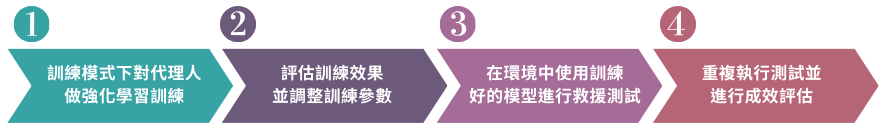
\includegraphics[width=\textwidth]{image/TrainingArch.png}
        \caption{實驗階段}
    \end{minipage}
\end{figure}

\newpage

\subsubsection{環境系統架構}
\begin{figure}[h]
    \centering
    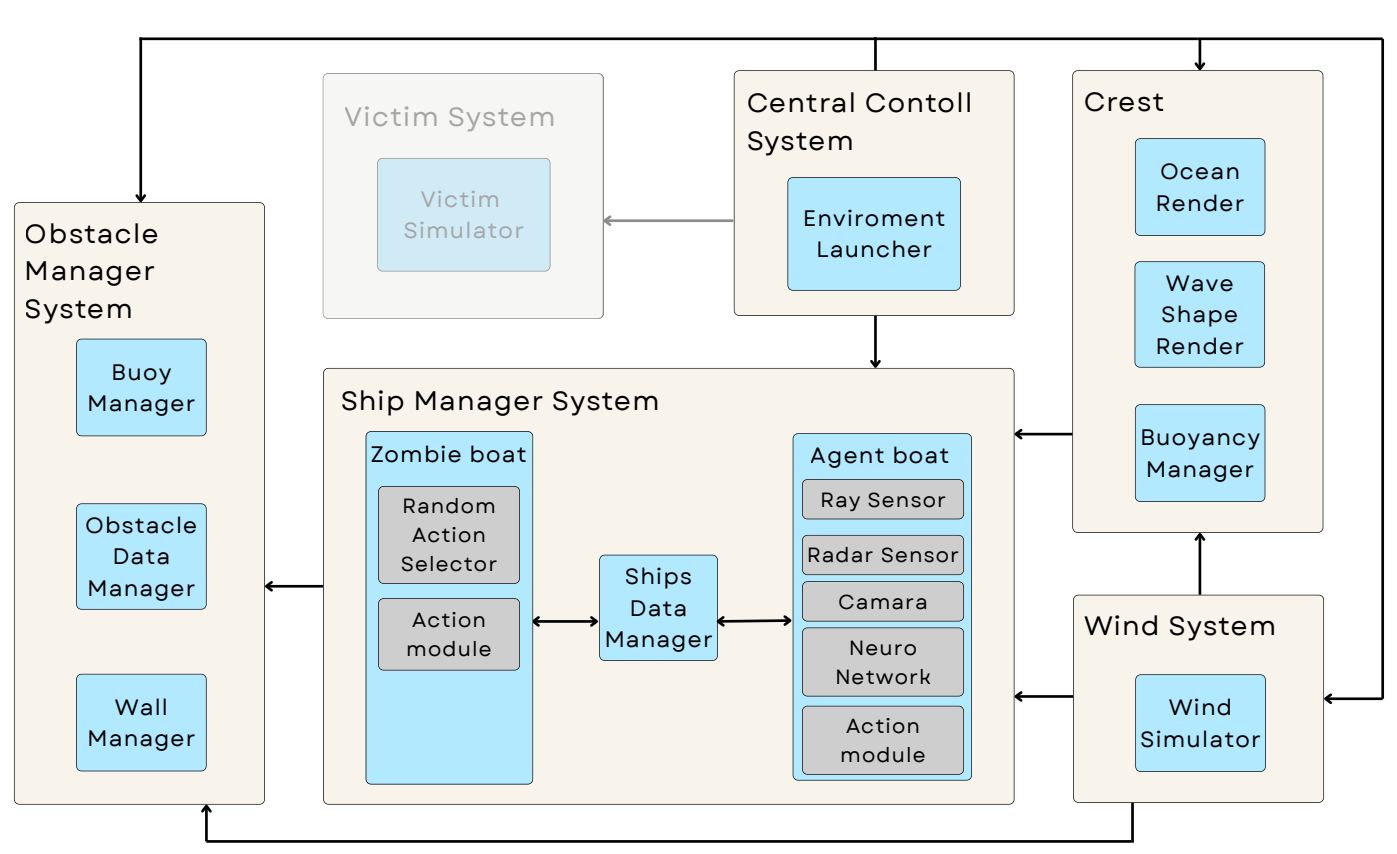
\includegraphics[scale=0.381]{image/TrainingArchitecture.png}
    \caption{訓練環境架構示意圖}
    \label{fig:training_env}

	\vspace*{0.3cm}

    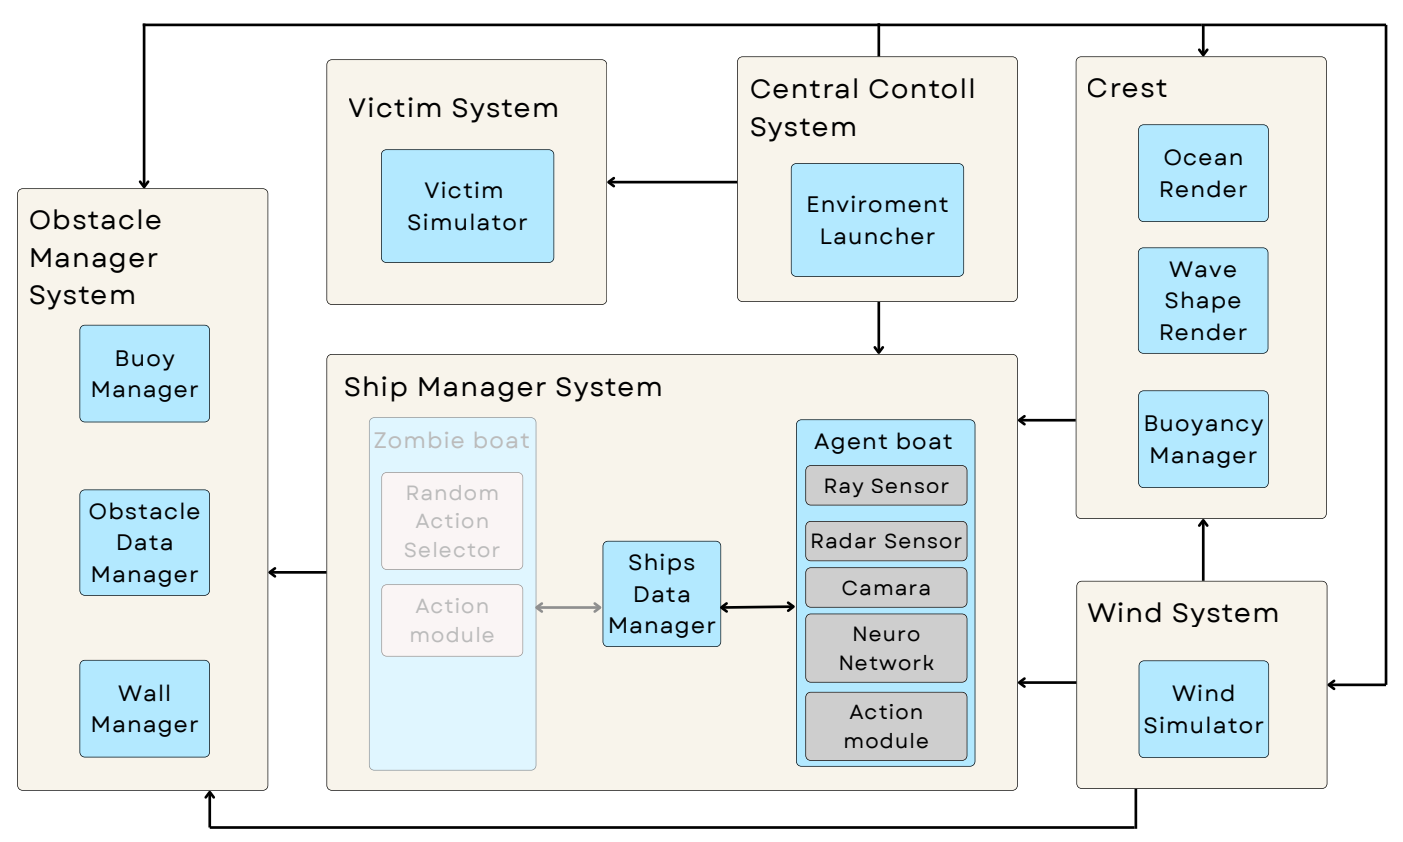
\includegraphics[scale=0.381]{image/SimulationArchitecture.png}
    \caption{模擬救援環境架構示意圖}
    \label{fig:simulation_env}
\end{figure}



\newpage

\begin{itemize}
	 \item \textbf{中央控制系統 (Central Control System)}
	\begin{itemize}
	    \item \textbf{環境啟動器 (Environment Launcher)}:負責啟動並管理整個環境。
	\end{itemize}
	
	 \item \textbf{船舶管理系統 (Ship Manager System)}
	\begin{itemize}
	    \item \textbf{殭屍船 (Zombie Boat)}:配備隨機動作選擇器與動作模組,作為訓練模式中的虛擬代理。
	    \item \textbf{智能船 (Agent Boat)}:訓練後的智能代理,配備射線感測器、雷達感測器、攝影機、神經網路與動作模組。
	    \item \textbf{船舶資料管理器 (Ships Data Manager)}:統一管理兩種船舶資料,例如當前位置、航向等。
	\end{itemize}
	
	 \item \textbf{波浪系統 (Crest)}
	\begin{itemize}
	    \item \textbf{海洋渲染器 (Ocean Render)}:負責生成整個海洋。
	    \item \textbf{波浪形狀渲染器 (Wave Shape Render)}:產生波浪的元件。
	    \item \textbf{浮力管理器 (Buoyancy Manager)}:處理物體在水中的浮力計算。
	\end{itemize}
	
	 \item \textbf{障礙物管理系統 (Obstacle Manager System)}
	\begin{itemize}
	    \item \textbf{浮標管理器 (Buoy Manager)}:生成及設定浮標參數,包括是否隨機、跟隨海浪飄移等。
	    \item \textbf{牆壁管理器 (Wall Manager)}:生成類牆壁障礙物。
	    \item \textbf{障礙物資料管理器 (Obstacle Data Manager)}:統一管理所有障礙物資料。
	\end{itemize}
	
	 \item \textbf{風力系統 (Wind System)}
	\begin{itemize}
	    \item \textbf{風力模擬器 (Wind Simulator)}:模擬海風,以重現更真實的搜救情境。
	\end{itemize}
	
	 \item \textbf{遇難者系統 (Victim System)}
	\begin{itemize}
	    \item \textbf{遇難者生成模擬器 (Victim Simulator)}:負責生成每次模擬中的遇難者。
	\end{itemize}
	
	 \item \textbf{系統與模組間的相互關係}
	\begin{itemize}
	    \item 船舶管理系統與障礙物管理系統互相溝通,避免碰撞。
	    \item 波浪系統影響船舶管理系統中船隻的物理特性。
	    \item 波浪系統影響障礙物管理系統中障礙物的物理特性。
	    \item 風力系統影響多個系統中各個物件的物理特性。
	\end{itemize}

\end{itemize}

\subsection{強化學習架構}

\subsubsection{觀測空間設計}
代理人的觀測空間包含四大類資訊:目的地資訊、船自身狀態、感測器資料以及其他船隻資訊。這些資訊能夠全面反映船隻的運動狀態、周遭環境以及目的地位置,使代理人在決策時具備充分的依據。

\paragraph{1. 目的地資訊 (3 維)}
\begin{itemize}
    \item 目的地方向(相對座標,2 維):將目的地相對於船隻的位置轉換至船體本地座標系,以 x、z 兩個分量表示水平方向。
    \item 與目的地的距離(1 維):計算船隻與目的地之間的歐氏距離,提供代理人對目的地接近程度的量化資訊。
\end{itemize}

\paragraph{2. 船自身狀態 (11 維)}
\begin{itemize}
    \item 速度 (3 維):x、z、y 分量,分別對應左右、前後及垂直方向的速度。
    \item 角速度 (3 維):偏航 (yaw)、翻滾 (roll) 與俯仰 (pitch) 三個方向的旋轉速度。
    \item 姿態資訊 (4 維):使用 roll 與 pitch 的正弦與餘弦值表示姿態。
    \item 剩餘步數 (1 維):記錄距離「每回訓練最大限制移動步數」的剩餘步數。
\end{itemize}

\paragraph{3. 感測器資料 (2n + 4 維)}
\begin{itemize}
	\item 障礙物感測器 (2n 維):將船周圍環境分為 n 個感測區段,每個區段提供距離最小障礙物的角度與距離。
	\item 海流感測 (2 維):
	\item 風向感測 (2 維):
\end{itemize}

\paragraph{4. 其他船隻資訊 (6m 維)}
\begin{itemize}
    \item 鄰近船隻狀態 (6m 維):對每艘鄰近船隻記錄相對方位角正弦/餘弦、距離、航向角正弦/餘弦、徑向速度。
\end{itemize}

\paragraph{5. 總結}
觀測空間總維度為:
\[
36 + 2n + 6m \text{ 維}
\]
其中 n 為感測區段數,m 為鄰近船隻數量。例如 n=8, m=3 時,總觀測空間為 52 維。

\newpage

\subsubsection{行動空間設計}
代理人的行動空間包含兩個連續控制維度:

\paragraph{1. 油門控制 (Throttle, 1 維)}
\begin{itemize}
\item 範圍:[-1.0, 1.0],正值向前推進、負值向後倒退,絕對值對應推進力強度
\item 功能:精細調整船隻加速度,實現平滑的速度控制
\end{itemize}

\paragraph{2. 舵向控制 (Steer, 1 維)}
\begin{itemize}
\item 範圍:[-1.0, 1.0],正值向右轉、負值向左轉,絕對值對應轉向力度
\item 功能:流暢調整航向,適應複雜的導航場景
\end{itemize}

\paragraph{3. 總結}
行動空間總維度為 2 維(油門 + 舵向)。此連續控制設計使代理人能夠同時控制速度與方向、達成精細的船隻控制,並模擬真實船隻操作,提升訓練策略的實用性。

\subsubsection{神經網路架構設計}

本研究的神經網路架構採用多模態輸入設計,結合視覺資訊與數值觀察,透過SAC演算法實現船舶的自主導航與避障能力。整體架構可分為輸入處理、特徵融合與決策輸出三個主要階段。

\vspace*{0.5cm}

\begin{figure}[h]
    \centering
    \begin{minipage}[t]{1\textwidth}
        \centering
        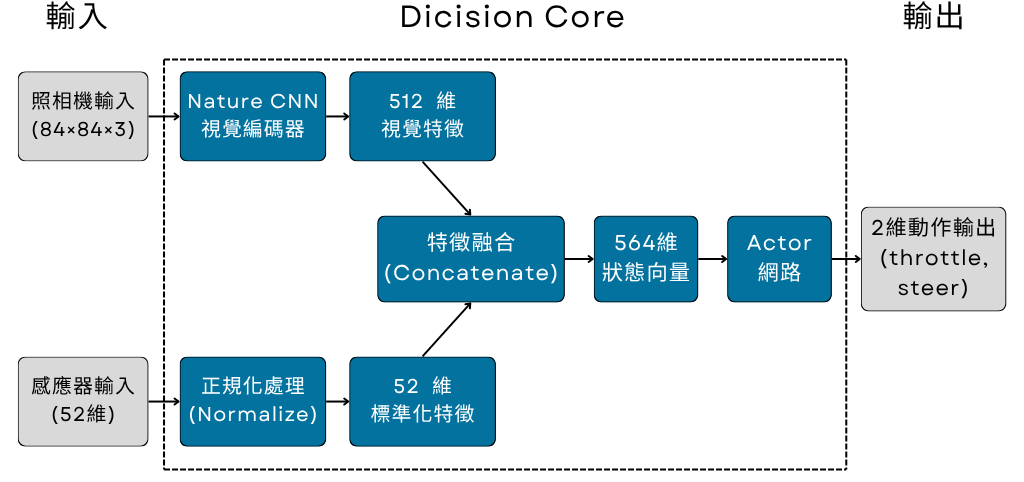
\includegraphics[width=\textwidth]{image/ModelArch.png}
        \caption{模型架構設計}
    \end{minipage}
\end{figure}

\paragraph{輸入處理階段}
\begin{itemize}
	\item \textbf{視覺輸入處理}:照相機提供$84\times84\times3$的RGB影像輸入,經由Nature CNN進行視覺特徵提取。Nature CNN採用三層卷積結構:第一層使用32個$8\times8$卷積核,步長為4,輸出$20\times20\times32$;第二層使用64個$4\times4$卷積核,步長為2,輸出$9\times9\times64$;第三層使用64個$3\times3$卷積核,步長為1,輸出$7\times7\times64$。經展平處理後得到3,136維特徵向量,再通過全連接層壓縮至512維視覺特徵向量。
	\item \textbf{數值觀察處理}:數值觀察空間包含52維特徵,涵蓋目標資訊(3維)、船隻運動狀態(11維)、感測器資料(20維)及其他船隻資訊(18維)。所有數值特徵經過正規化處理,使用運行平均值與標準差進行標準化:
\end{itemize}

\begin{equation}
\text{normalized\_value} = \frac{\text{original\_value} - \text{running\_mean}}{\sqrt{\text{running\_variance} + 10^{-8}}}
\end{equation}

\paragraph{特徵融合階段}

視覺特徵向量(512維)與標準化數值向量(52維)透過連接操作融合為560維的綜合特徵向量,作為SAC演算法的輸入狀態表示。

\paragraph{SAC神經網路架構}
\begin{itemize}

	\item \textbf{Actor網路(策略網路)}:輸入560維融合特徵,經過三層隱藏層處理,每層包含256個神經元並使用ReLU激活函數。輸出層產生2維連續動作向量,分別控制船隻的油門(throttle)與轉向(steer),動作範圍為$[-1, 1]$。
	
	\item \textbf{Critic網路(價值網路)}:採用 twin Q-networks 架構\cite{Atari}提升訓練穩定性。每個 Q-networks 接收560維狀態特徵與2維動作輸入,總輸入維度為562。網路結構與 Actor 相同,使用三層256個神經元的隱藏層,輸出單一Q值估計。
	
	\item \textbf{目標網路與熵正則化}:系統維護Actor與Critic的目標網路副本,透過軟更新機制($\tau=0.01$)逐步同步參數。SAC演算法引入熵正則化項,初始熵係數設為0.1,透過自動調整平衡探索與利用。
\end{itemize}

\paragraph{網路訓練配置}

訓練過程採用Adam optimizer,學習率設為$5\times10^{-5}$,批次大小256,經驗回放緩衝區容量300,000。折扣因子$\gamma$設為0.99,最大訓練步數為400,000步,時間範圍設定為300步。

\paragraph{架構特點總結}

本架構的核心特點包括:多模態融合設計能有效結合視覺與數值資訊;Nature CNN專門處理空間視覺特徵;數值正規化確保不同尺度特徵的平衡學習;SAC演算法的最大熵特性平衡探索與利用;twin Q-networks 設計提升價值估計穩定性。整體參數量約162萬個,能夠在複雜海洋環境中實現穩定的自主導航性能。

\subsubsection{獎勵函數設計}

本研究所設計的強化學習獎勵系統,旨在引導船隻在模擬環境中安全且高效地到達目標位置。總獎勵 $R_t$ 由兩部分組成:持續獎勵 $R_{\text{cont}}$ 與終止情況的額外獎勵 $R_{\text{terminal}}$。其中,持續獎勵提供船隻行為的即時指導信號,而終止獎懲則針對明確事件給予強烈反饋。

\paragraph{1. 持續獎勵}
持續獎勵由三個子項組成:
\begin{itemize}
    \item \textbf{距離進展獎勵 (Distance Progress Reward)}:
    \[
    r_{\text{dist}} = R_D \cdot \tanh(3 \Delta d), \quad \Delta d = d_{t-1}-d_t
    \]
    \item \textbf{航向獎勵 (Heading Reward)}:
    \[
    r_{\text{head}} = R_H \cdot (f \cdot u)
    \]
    \item \textbf{障礙物懲罰 (Proximity Penalty)}:
    \[
    r_{\text{prox}} = R_P^{\max} \cdot \max\!\left(0, \frac{W - m_t}{W}\right)
    \]
\end{itemize}

\paragraph{2. 終止情況的額外獎勵}
\begin{itemize}
    \item \textbf{成功到達目標 (Success Reward)}:
    \[
    R_{\text{succ}} + r_{\text{time}}, \quad
    r_{\text{time}} = \max\!\left(0, \frac{T_{\max}-s}{T_{\max}}\right) R_{\text{tb}}^{\max}, \quad d_t<d_{\text{succ}}
    \]
    \item \textbf{碰撞 (Collision Penalty)}:
    \[
    R_{\text{col}}, \quad m_t < m_{\text{col}}
    \]
    \item \textbf{超時 (Timeout Penalty)}:
    \[
    R_{\text{to}}, \quad s > T_{\max}
    \]
\end{itemize}

\paragraph{3. 總獎勵}
每一步的總獎勵為:
\[
R_t = R_{\text{cont}} + R_{\text{terminal}}
\]

其中,持續獎勵為:
\[
R_{\text{cont}} = r_{\text{dist}} + r_{\text{head}} + r_{\text{prox}}
\]

終止情況的額外獎勵為:
\[
R_{\text{terminal}} =
\begin{cases}
R_{\text{col}}, & m_t < m_{\text{col}} \\
R_{\text{succ}} + r_{\text{time}}, & d_t < d_{\text{succ}} \\
R_{\text{to}}, & s > T_{\max} \\
0, & \text{其他情況}
\end{cases}
\]

綜合總獎勵公式:
\[
\begin{aligned}
R_t &= R_D \tanh(3 \Delta d) + R_H (f \cdot u) + R_P^{\max} \max\!\Big(0,\frac{W-m_t}{W}\Big) \\
&\quad +
\begin{cases}
R_{\text{col}}, & m_t < m_{\text{col}}\\
R_{\text{succ}} + \displaystyle \max\!\Big(0,\frac{T_{\max}-s}{T_{\max}}\Big) R_{\text{tb}}^{\max}, & d_t < d_{\text{succ}}\\
R_{\text{to}}, & s > T_{\max}\\
0, & \text{otherwise}
\end{cases}
\end{aligned}
\]

\renewcommand{\arraystretch}{1.3} % 調整表格行距
\begin{table}[h!]
\centering
\begin{minipage}{0.48\textwidth}
\centering
\caption{符號定義}
\vspace*{0.2cm}
\begin{tabular}{ll}
\hline
\textbf{符號} & \textbf{定義} \\
\hline
$d_t$ & 當前時間步到目標的距離 \\
$d_{t-1}$ & 上一時間步到目標的距離 \\
$\Delta d$ & $d_{t-1} - d_t$ \\
$m_t$ & 最小障礙物距離 \\
$W$ & 障礙物警戒距離 \\
$s$ & 當前步數 (StepCount) \\
$T_{\max}$ & timeout 上限 \\
$f$ & 船的前向單位向量 \\
$u$ & 船到目標的單位向量 \\
\hline
\end{tabular}
\end{minipage}
\hfill
\begin{minipage}{0.48\textwidth}
\centering
\caption{常數設定(程式內數值)}
\vspace*{0.2cm}
\begin{tabular}{ll}
\hline
\textbf{常數} & \textbf{數值與說明} \\
\hline
$R_D$ & 1.0,距離獎勵係數 \\
$R_H$ & 0.2,航向獎勵係數 \\
$R_P^{\max}$ & -0.3,障礙物最大懲罰 \\
$W$ & 15,警戒距離 \\
$R_{\text{succ}}$ & 1.0,成功獎勵 \\
$R_{\text{col}}$ & -1.0,碰撞懲罰 \\
$R_{\text{to}}$ & -0.6,超時懲罰 \\
$R_{\text{tb}}^{\max}$ & 0.4,時間獎勵最大值 \\
$m_{\text{col}}$ & 0.8,碰撞閾值 \\
$d_{\text{succ}}$ & 5,成功閾值 \\
\hline
\end{tabular}
\end{minipage}
\end{table}

\newpage

\section{實驗設計與結果分析}

\subsection{實驗環境架設}
本實驗的模擬環境由 Unity 遊戲引擎及 Crest 海洋物理引擎結合而成,得以表現出真實的海面動態與船舶的物理特性。為測試自主船舶在不同情境下的效能,我們在環境中加入了多個變因:
\begin{itemize}
    \item 遇難者的位置:單個或隨機生成
    \item 動態障礙物:漂浮物、其他搜救船隻等
    \item 搜索區域大小與分塊方式
\end{itemize}
透過上述條件組合與調整,我們得以評估自主船舶在海洋環境中的表現與穩定性。

\subsection{模型訓練概述}
\subsubsection{訓練目標}
我們使用 SAC 深度強化學習演算法進行模擬訓練,旨在讓自主船舶具有導航能力與穩定避障的能力。因此在訓練的過程中,我們特別重視船舶的兩種指標:
\begin{itemize}
    \item 任務完成時長:船隻由初始位置到目標點所需時間
    \item 碰撞次數:船隻與障礙物碰撞次數
\end{itemize}
訓練過程中,我們著重於降低兩者的數值,以確保船舶能在多變且複雜的條件下能夠維持良好的表現,並且得以完成任務目標。

\subsubsection{訓練環境的架設}
本實驗的訓練環境以 Unity 與 Crest 海洋物理引擎為基礎,模擬出真實的海面,包括風浪、風速及動態的障礙物,以提供船隻導航及避障所需的複雜環境。我們在場景中配置一個訓練船隻,並加入多艘「殭屍船」作為其他代理人的替代品,這些船隻會隨機行動,模擬多代理系統的互動行為。
值得注意的是,雖然整體系統設計為多代理人系統,但直接訓練多代理人系統會使環境過於複雜,使收斂時間過長,甚至可能無法收斂,而我們的訓練目標僅是船隻的避障與導航,不會涉及代理間的合作。因此我們採用了單代理人的訓練方式,結合上述的「殭屍船」模擬多代理環境,既能節省資源,又能讓代理學習多代理系統下的避障與導航策略。

\newpage

\subsubsection{訓練流程}
我們的訓練環境以 Unity 與 Crest 為主,結合 ML-Agents 深度強化學習框架,讓自主船舶能在真實的海面條件下學習避障與導航能力。整個流程可以分為以下階段:
\begin{enumerate}
    \item \textbf{環境初始化}:配置船隻、目標點、障礙物與 「殭屍船」。
    \item \textbf{深度強化學習訓練}:透過 ML-Agents 啟動訓練流程,並採用 SAC 演算法進行訓練,訓練目標為讓船隻從初始位置移動到目標點,同時,在途中不能碰到障礙物或是「殭屍船」。
    \item \textbf{訓練監控與紀錄}:使用 TensorBoard 監控訓練過程,包括回合獎勵、碰撞事件與成功到達目的地的次數。
    \item \textbf{模型測試與驗證}:將訓練完成的模型部屬於模擬場景中,測試其在不同環境下的避障與導航表現。
    \item \textbf{結果分析與策略優化}:根據訓練與測試的結果,分析模型在各方面的效能。
\end{enumerate}

\begin{figure}[h]
    \centering
    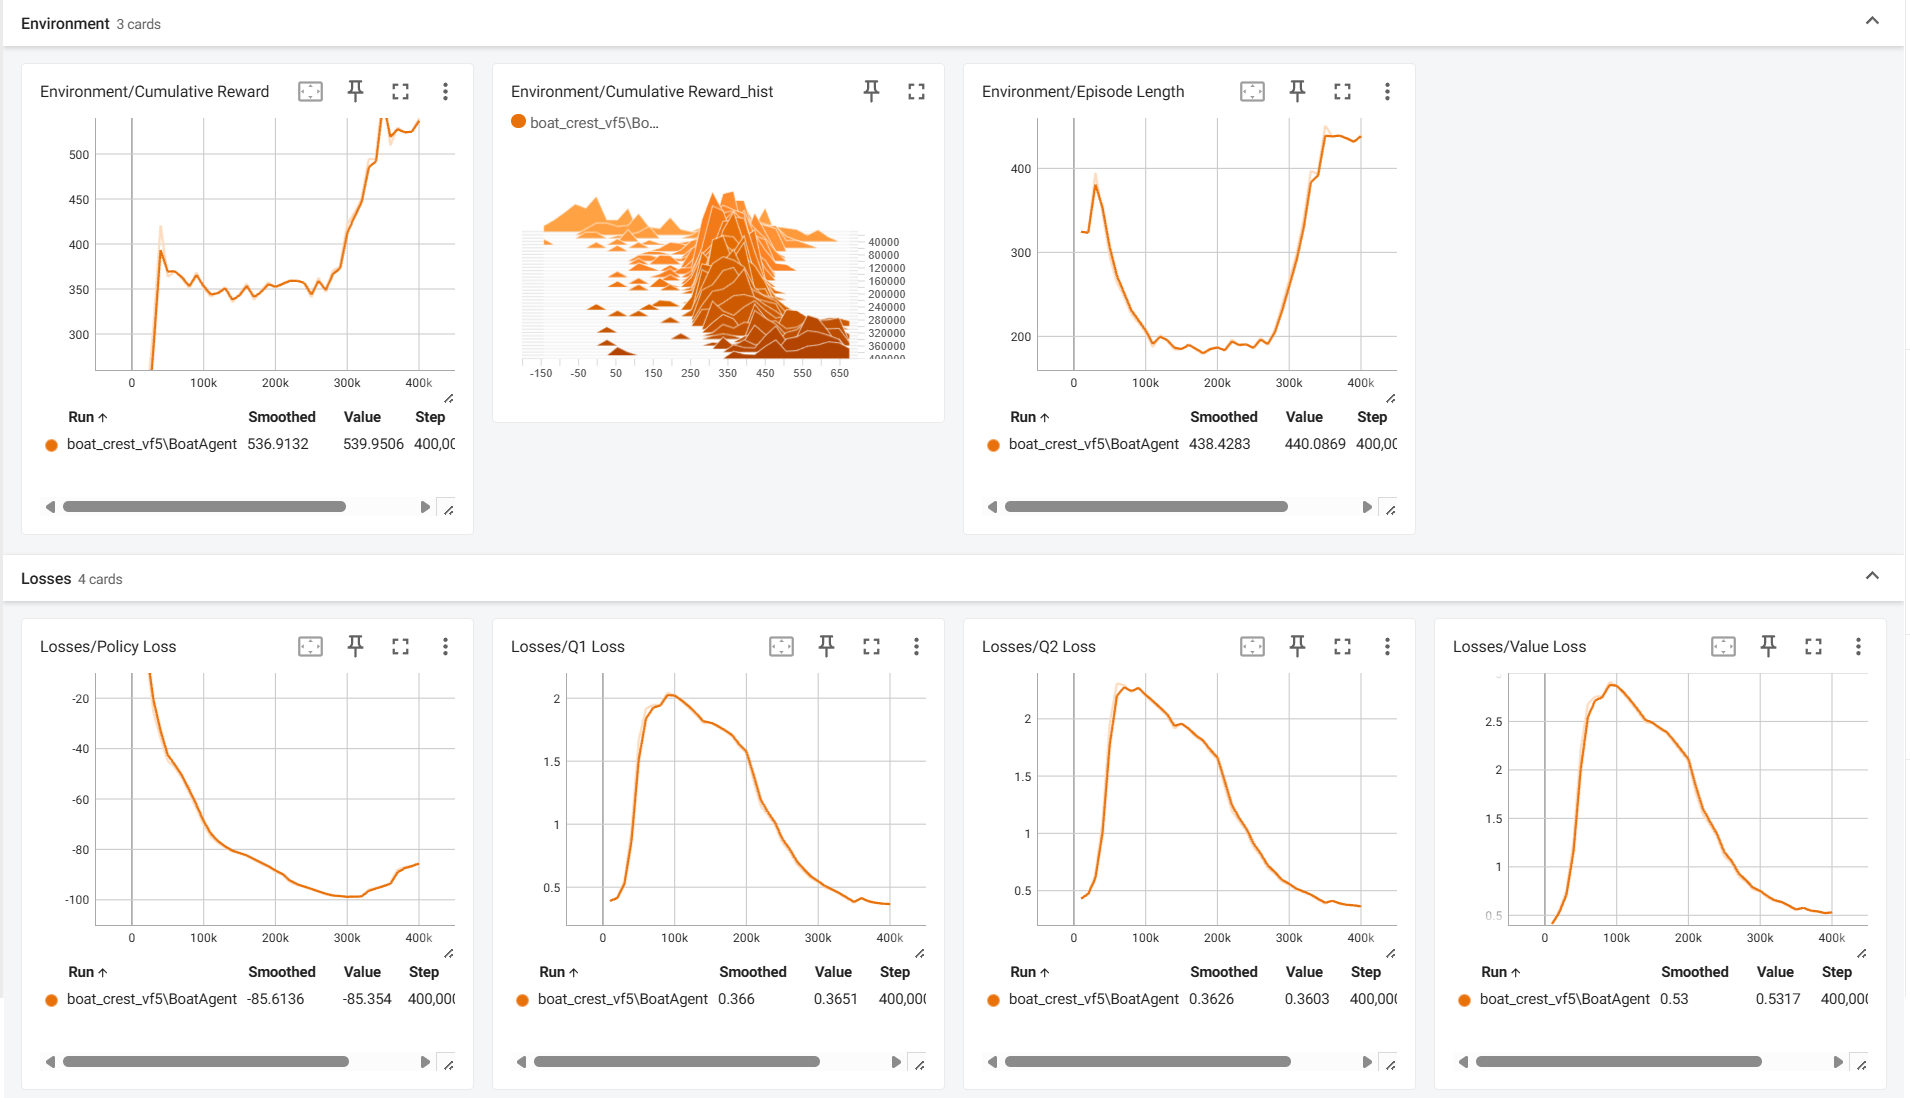
\includegraphics[scale=0.3]{image/Tensorboard.png}
    \caption{Tensorboard 訓練結果示意圖}
\end{figure}

\subsection{模擬任務設計與測試方法}
自主船舶在經過深度強化學習的訓練後,已經具備了導航能力與避障能力,這使船舶能夠執行更高層次的任務—搜尋與救援。我們在設計過程中選擇了最為直觀的方法—\textbf{平行線搜尋法}\cite{IAMSAR2008}。這種方法透過多搜船舶同時沿著平行航線推進,在大範圍的區域內進行高覆蓋率的搜尋,以擴大搜尋範圍並降低遺漏目標的可能性。雖然在傳統上,平行線搜尋法相較其他搜尋方法需要更大量的人力與資源,但本實驗所提出的自主船舶系統能夠以更低的成本執行此策略,並利用群集間的偕同航行來擴大搜尋範圍。

\subsubsection{單一落水點快速救援}
這個情景用來模擬單一人員落海的情況,例如郵輪乘客落海、近岸游泳者被離岸流捲走、或是小型漁船翻覆導致單人落水等情景。該情境強調時間的敏感性及位置的不確定性,船隊需要經過仔細的搜尋,在最快的時間內定位落水的人員,並進行施救,而系統需要根據當前的海流資料,預測人員的出現位置範圍,並引導船隊前去搜救。
\\ \par
在這個情景下,我們使用以下方法設定我們的環境:
\begin{itemize}
    \item 遇難者定位:位置不明,只知道大概的範圍。
    \item 測試參數:
    \begin{itemize}
        \item 偵測半徑:100 m
        \item 船隻數量:5 艘
        \item time-out:200 秒
        \item 障礙物密集度:無障礙物
    \end{itemize}
    \item 終止條件與成功判定:
    \begin{itemize}
        \item 成功:任一船隻找到落水者並標記,在 time-out 前完成。
        \item 終止:超過 time-out、發生嚴重碰撞等。
    \end{itemize}
    \item 示意圖
	\begin{figure}[h]
	    \centering
	    \begin{minipage}[t]{0.55\textwidth}
	        \vspace{1cm} 
	        \textbf{示意圖說明:}\\
	        此圖展示了模擬情況下進行單一落水點快速救援的情境。\\
	        下方排列四艘船隻,模擬開始時會開始向前掃描,於系統訂定的搜尋範圍內找尋落水人員。上方的亮點為落水人員,等待被施救。\\
		此圖僅為示意圖,真實的模擬情境船隻間距會更寬廣一些,落水人員不會距離船隊這麼近。
	    \end{minipage}
	    \hfill
	    % 右側圖片
	    \begin{minipage}[t]{0.4\textwidth}
	        \vspace{0pt}
	        \centering
	        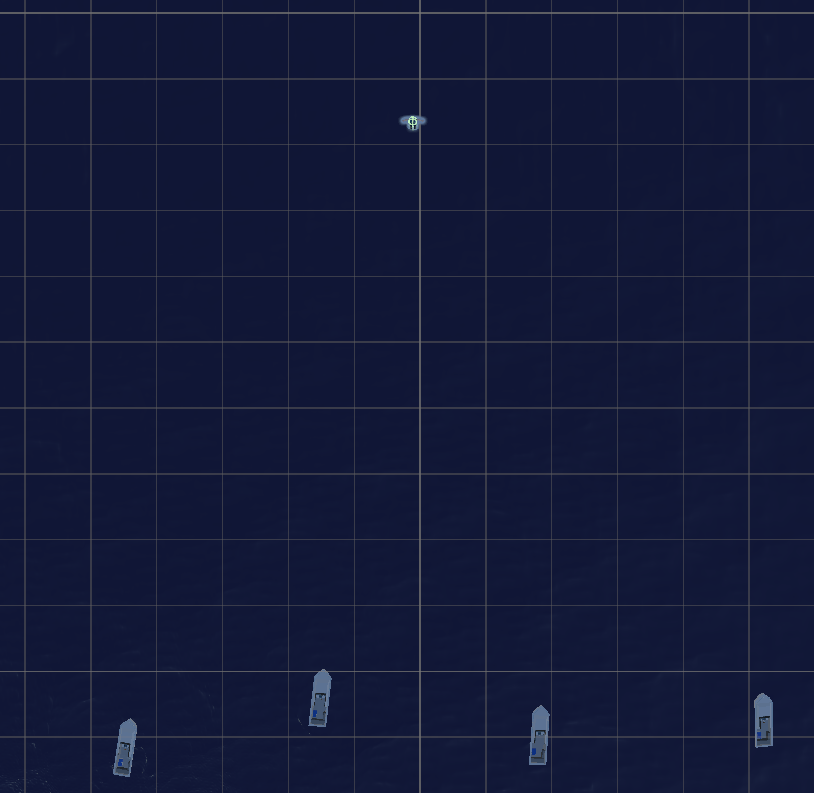
\includegraphics[width=\textwidth]{image/SingleDemo.png}
	        \caption{單一搜尋示意圖}
	    \end{minipage}
	\end{figure}

\end{itemize}

\newpage

\subsubsection{大範圍隨機搜尋任務}
此情景用來模擬在大面積海域中進行隨機分布的搜救任務,例如海上船舶遇難、飛機海面迫降等等。該情境除了強調搜尋的覆蓋範圍與船體之間的配合外,更著重於船舶是否可以躲避各種飛機、船舶的碎片。船隊需要在目標數量與位置不明確的情況下,盡可能的提高搜尋效率與範圍覆蓋率,同時也要降低碰撞的風險。
\\ \par
在這個情景下,我們使用以下的方法設定模擬環境:
\begin{itemize}
    \item 目標分布:多個目標隨機生成於整個搜索區域,位置與數量隨機。
    \item 測試參數:
    \begin{itemize}
        \item 偵測半徑:125 m
        \item 船隻數量:5 艘
        \item time-out:200 秒
        \item 障礙物密集度:每平方公里 500 個
        \item 落海人數:10 人
    \end{itemize}
    \item 終止條件與成功判定:
    \begin{itemize}
        \item 成功:船隻找到所有落水人員並標記,在 time-out 前完成。
        \item 終止:超過 time-out、發生嚴重碰撞等。
    \end{itemize}
    \item 示意圖
\end{itemize}
\begin{figure}[h]
    \begin{minipage}[t]{0.55\textwidth}
        \vspace{1cm} 
        \textbf{示意圖說明:}\\
	右圖呈現了模擬環境下進行大範圍隨機搜尋任務的情境。\\
	此情境模擬大型船難事故,乘客隨機散落於海面各處,船隊則採用與單一落水點相同的平行線搜尋策略,逐一搜尋並標記遇難者,以便救援人員後續施救。
	圖中僅示範單一船舶的視角,可清楚觀察到海面上分布著多名待救援人員。
    \end{minipage}
    \hspace{2em}
    \begin{minipage}[t]{0.45\textwidth}
        \vspace{0pt}
        \centering
        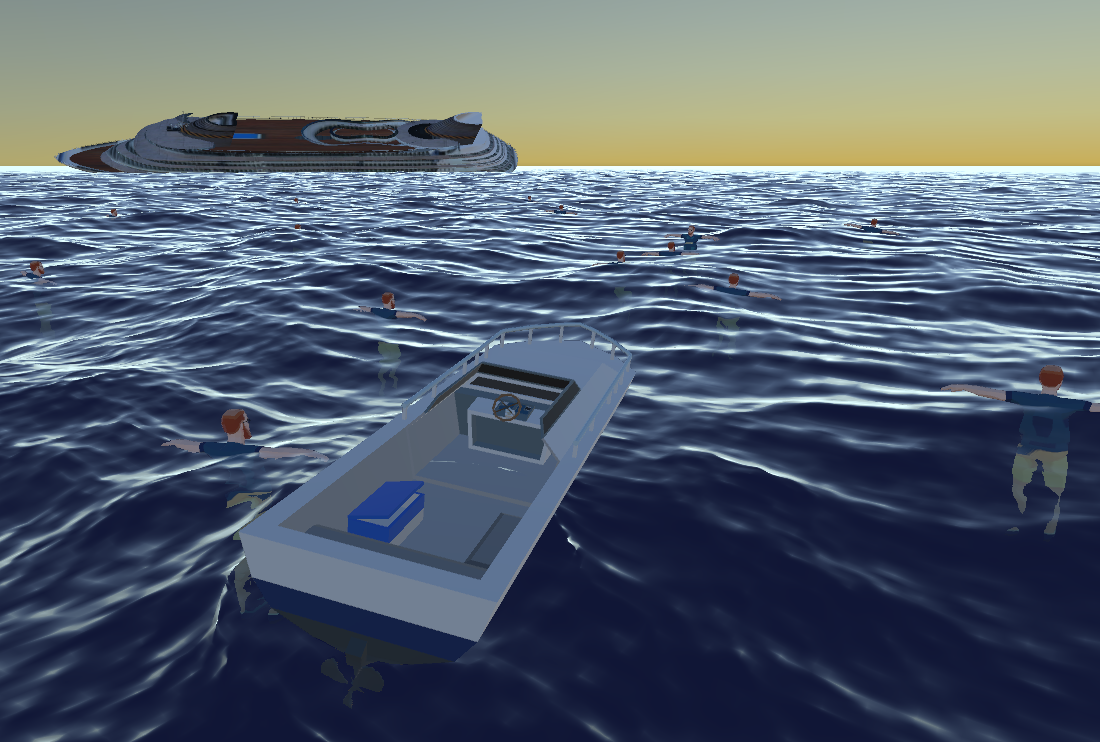
\includegraphics[width=\textwidth]{image/MultiDemo.png}
        \caption{大範圍搜尋示意圖}
    \end{minipage}
\end{figure}

\newpage

\subsubsection{任務效能評估}
有了以上兩種情境後,我們根據我們的需求制定了一系列的評估指標來量化船隊在搜尋任務中的表現。主要指標包括:
\begin{itemize}
    \item \textbf{成功救援率}:在任務時間的限制內,船隊成功找到落水者的比例。
    \item \textbf{搜尋覆蓋程度}:船隊在搜尋任務中實際搜尋的範圍。
    \item \textbf{預測成功率}:在單一落水點快速救援時,一次模擬結束時,人員位在系統預測範圍內的比率。
\end{itemize}

以上的指標除了量化船隊在救援上的表現外,也同時得以反映任務中錯誤的發生率。透過對這些指標進行系統化的分析,我們設計了以下的終極目標,以確保在實際應用中既能提高救援效率,又能控制風險與資源消耗:
\begin{itemize}
    \item \textbf{提高成功救援率}:增加船隊的可靠性及穩定性。
    \item \textbf{提高搜尋覆蓋程度}:確保區域被充分搜尋,降低目標遺漏的機率。
    \item \textbf{提高預測成功率}:確保系統能預測落水人員的位置。
\end{itemize}

\subsubsection{測試流程}
\begin{enumerate}
    \item 根據以上兩種情境設定參數:包括船隻數量、偵測半徑、障礙物密度等等,確保模擬場景能夠模擬出多種真實情況。
    \item 部屬船隊於初始位置準備開始:船隻將自行到達初始位置,並等待所有船隻就位,確保所有船隻同時開始搜尋。
    \item 開始進行搜尋,每艘船分別執行合作搜尋任務:船隊依據既定的策略及路徑,開始進行搜尋,過程中系統根據目前的搜尋範圍,規劃所有船隻的走向。
    \item 紀錄相關數據以利未來做分析。例如:各艘船時間-位置關係、風向與環境參數、落水人員的預估範圍、總搜救時間、成功救援的人員數量。
    \item 重複模擬多次,以獲取大量數據進行分析:透過不同的環境重複實驗,確保結果可靠,並進行進一步的分析。
\end{enumerate}

\newpage

\subsection{測試結果呈現}
\subsubsection{單一落水點快速救援}

以下四張圖展示了搜尋任務的執行過程,依時間順序排列。圖中圓圈表示系統推測的落水者可能位置範圍,而紅色叉號則標示實際遇難者所在位置。不同顏色的區塊代表各艘船隻在搜尋過程中對不同區域的覆蓋次數,顯示搜尋頻率與範圍。由於落水者可能會隨海流移動,系統會即時估計其當前位置,並將紅圈調整至對應位置。船隊自圖中左下角出發,並根據推測的落水範圍展開搜尋策略。

\begin{figure}[h]
    \centering
    % 第一排
    \begin{minipage}[t]{0.45\textwidth}
        \centering
        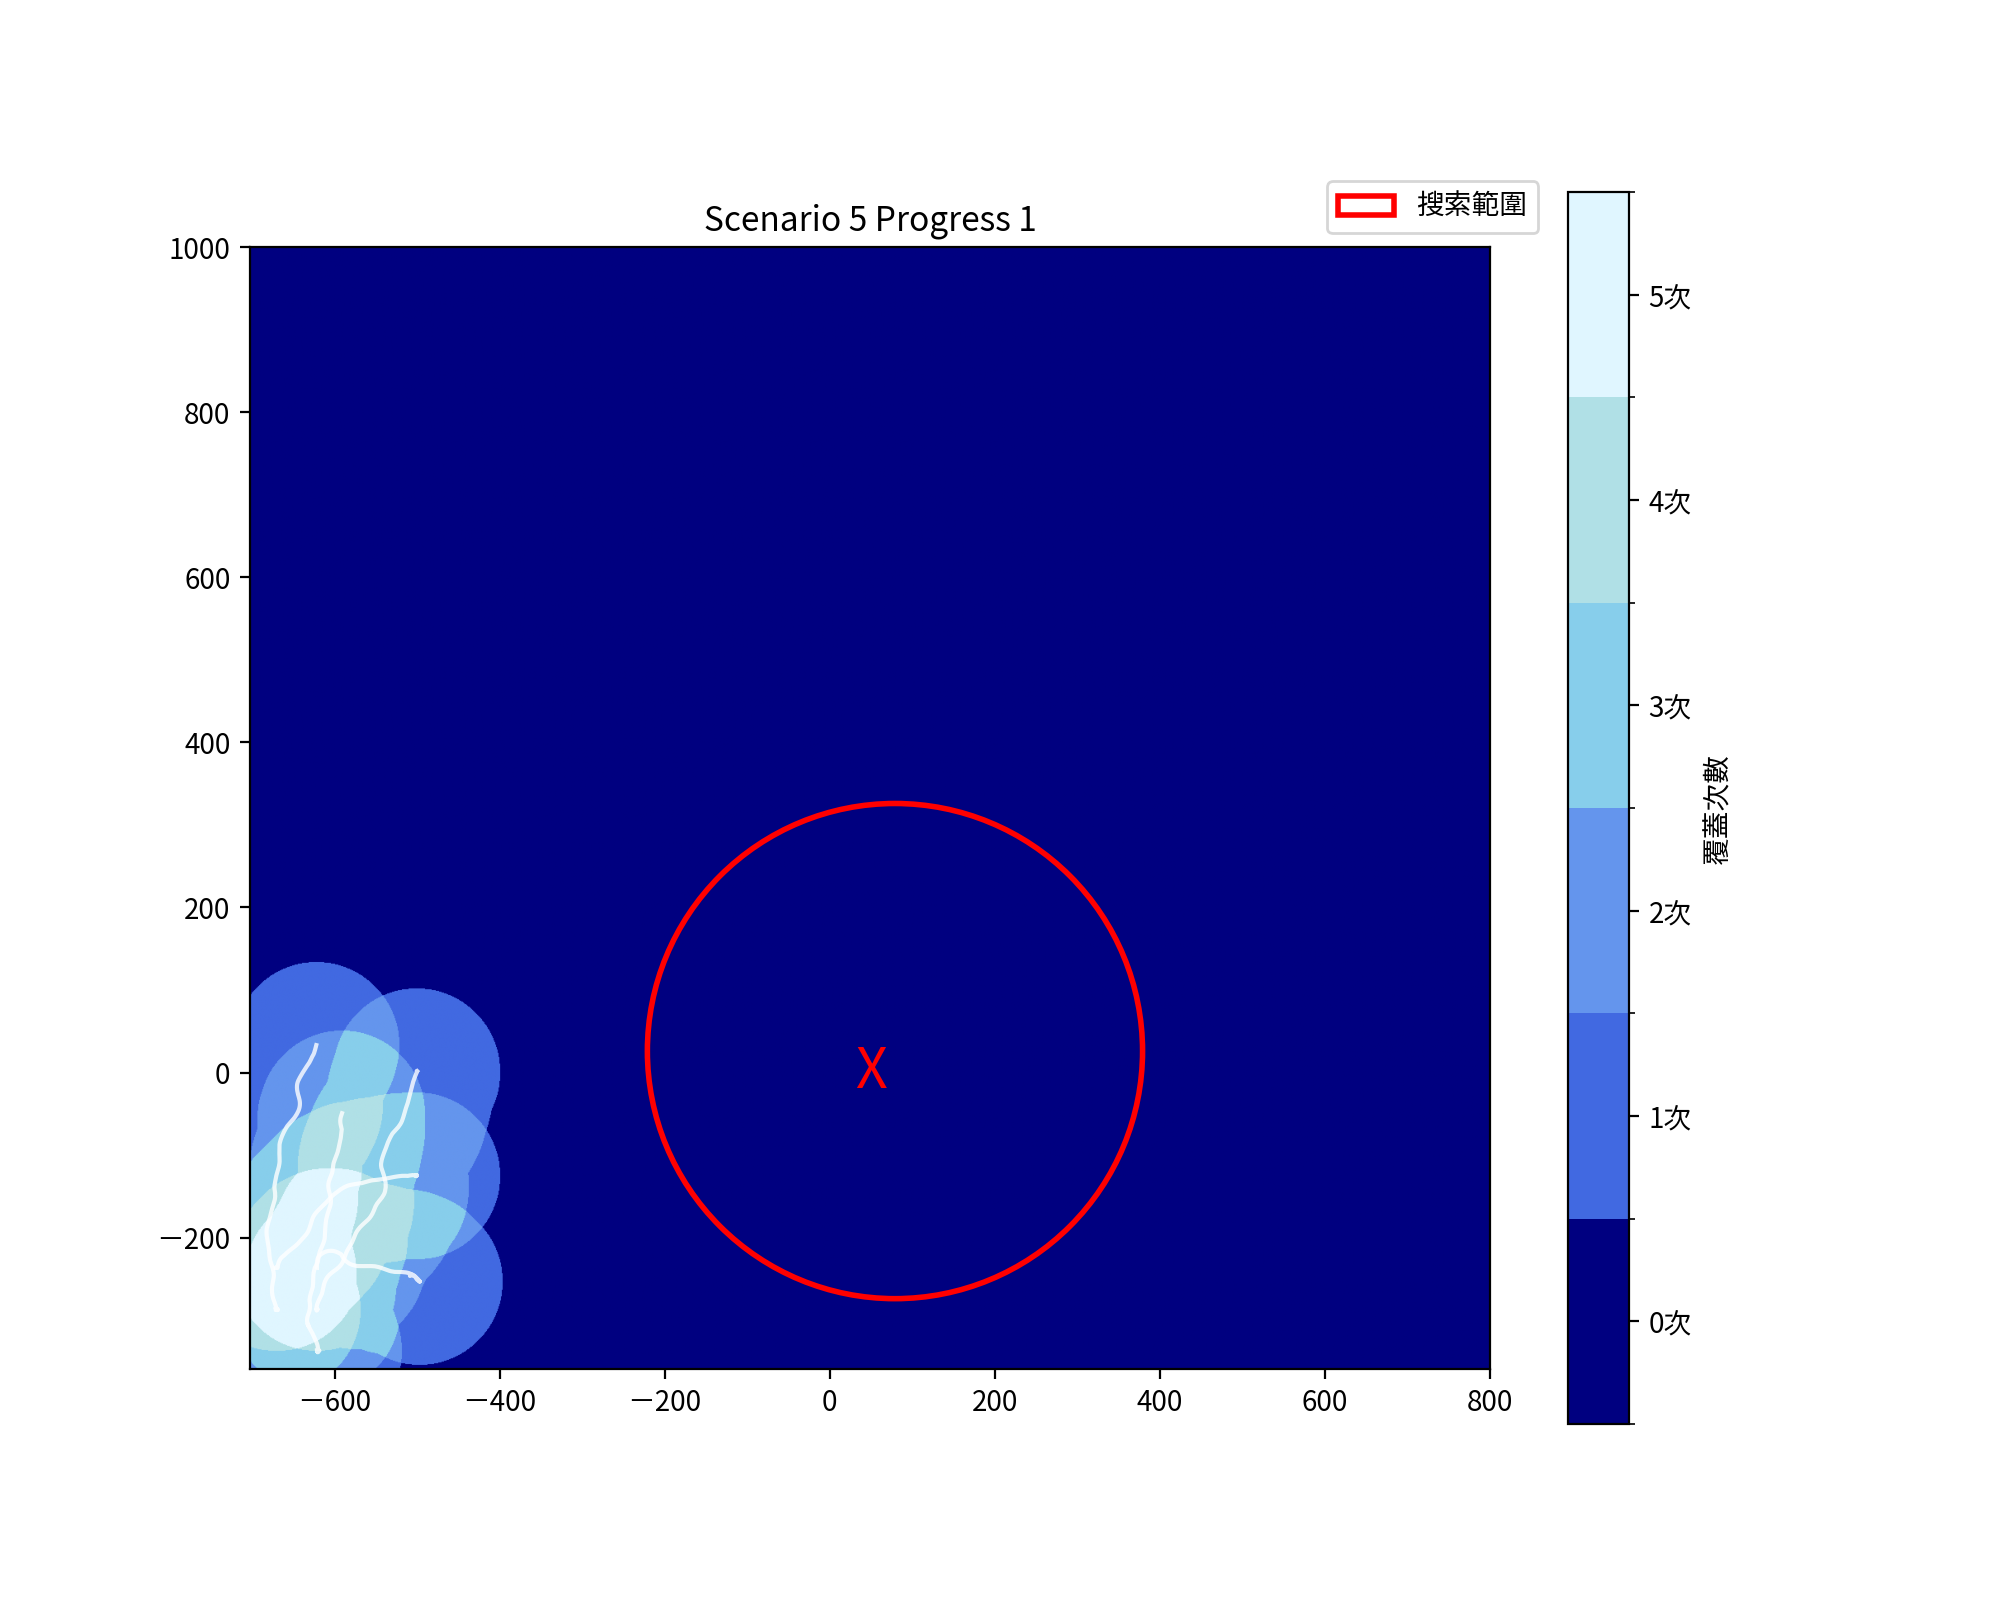
\includegraphics[width=\textwidth]{image/Single1.png}
        \caption{搜尋進度一}
    \end{minipage}
    \hfill
    \begin{minipage}[t]{0.45\textwidth}
        \centering
        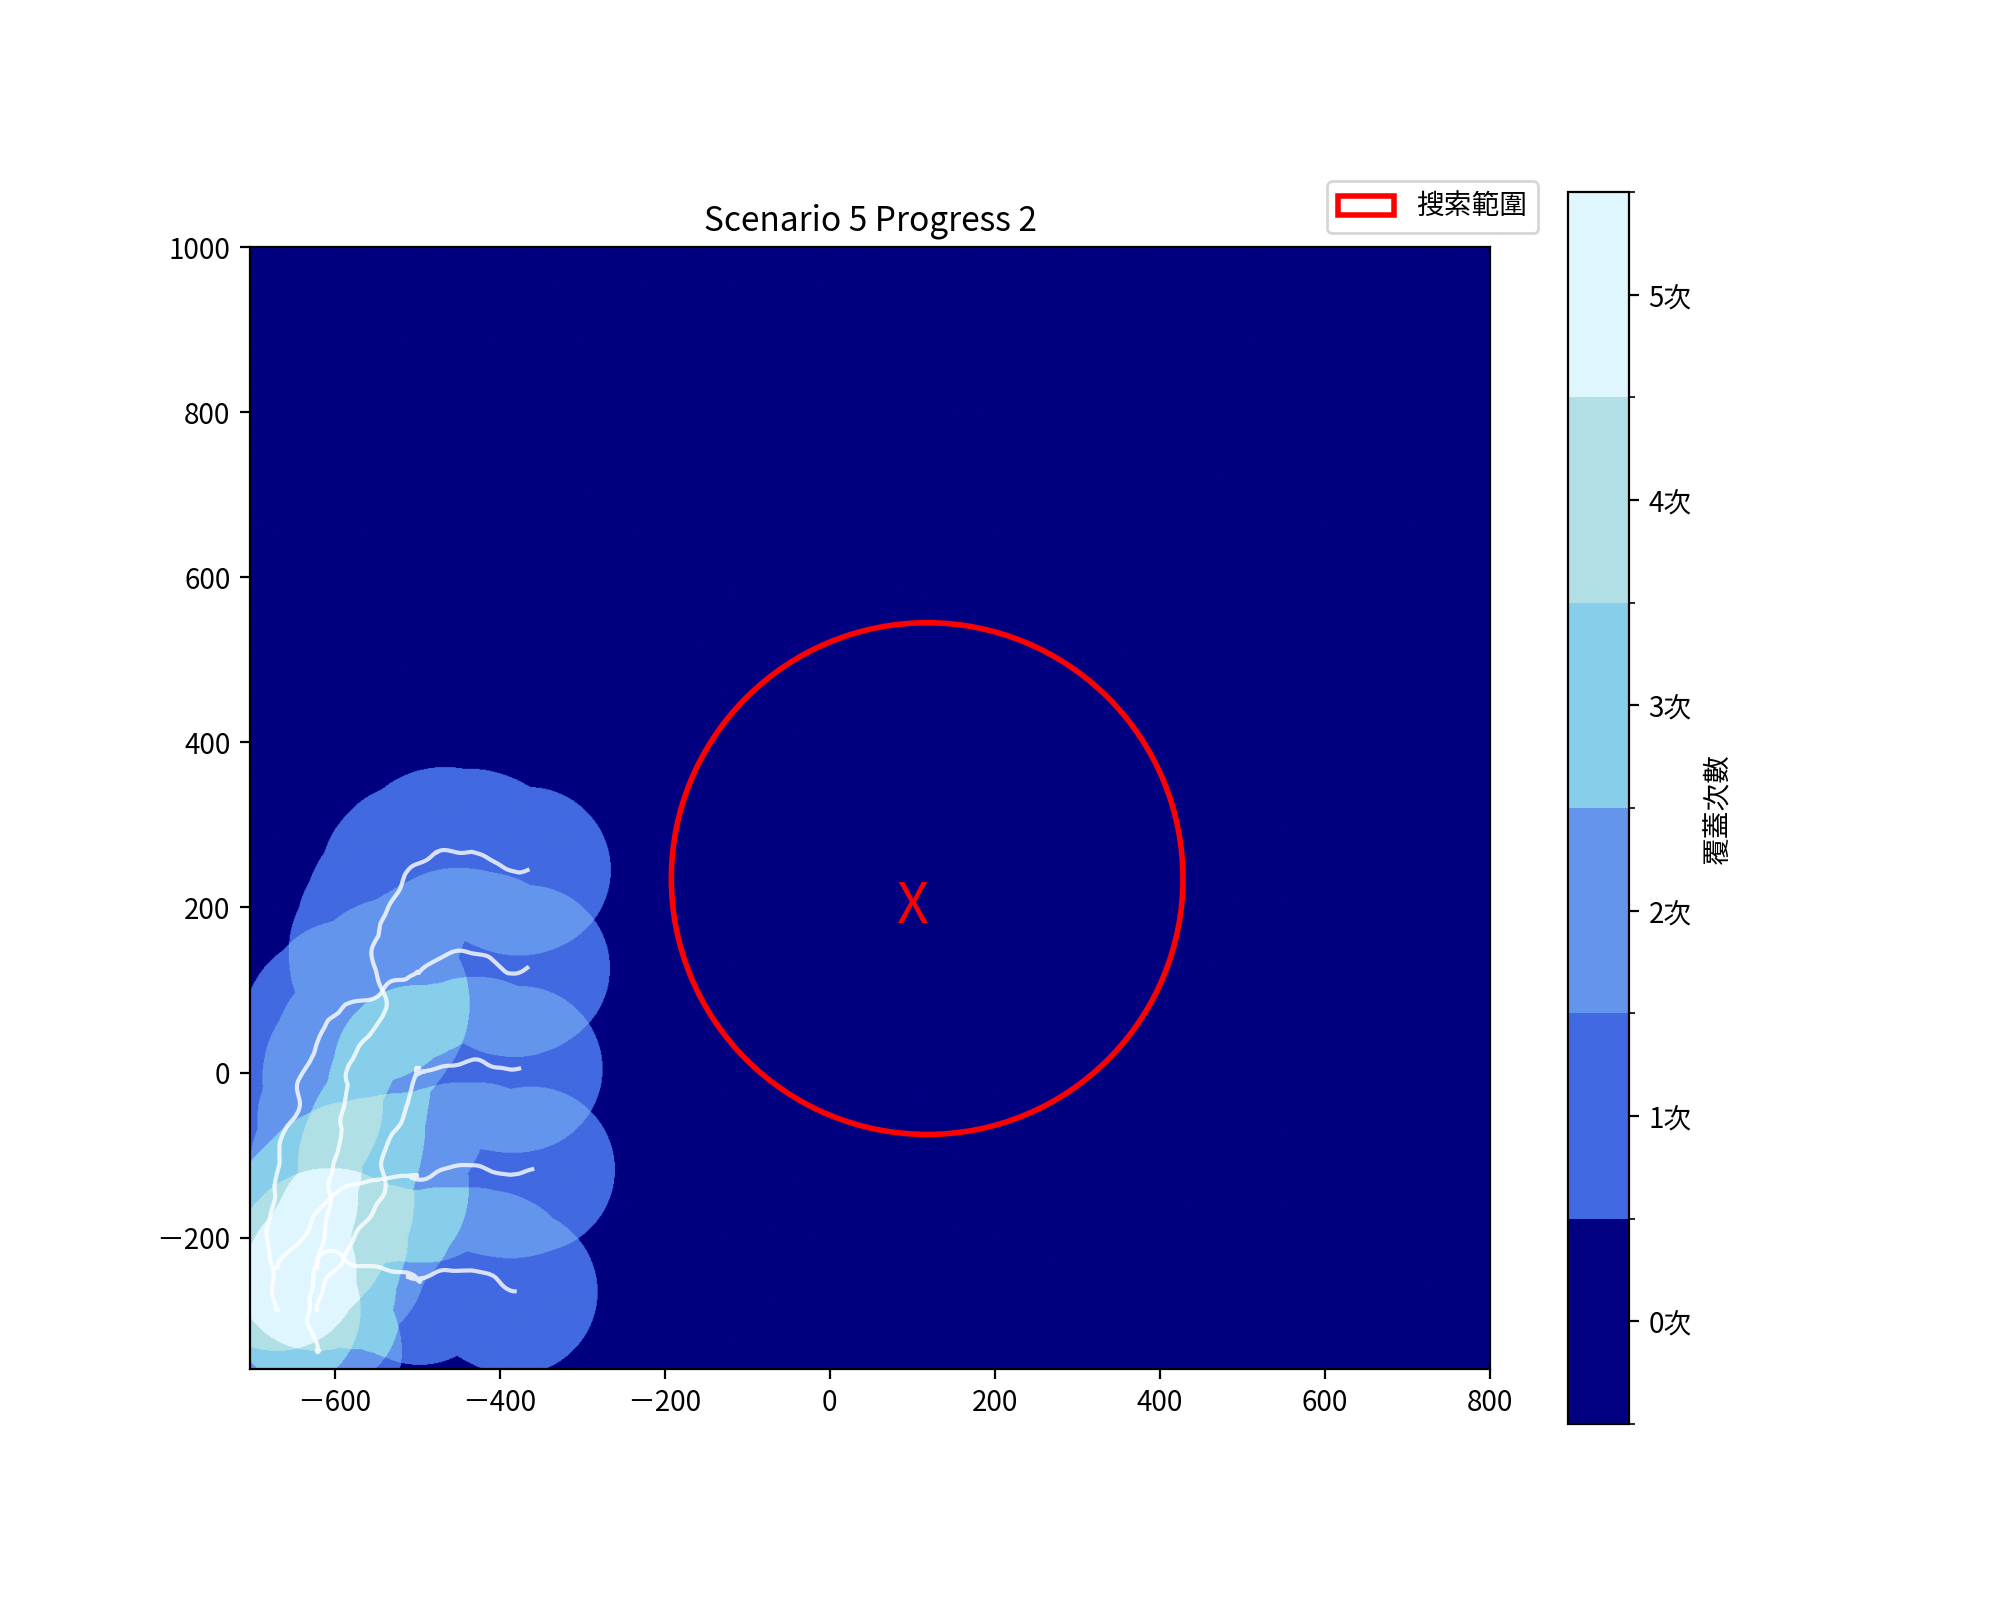
\includegraphics[width=\textwidth]{image/Single2.png}
        \caption{搜尋進度二}
    \end{minipage}

    \vspace{0.5em} % 換行間距

    % 第二排
    \begin{minipage}[t]{0.45\textwidth}
        \centering
        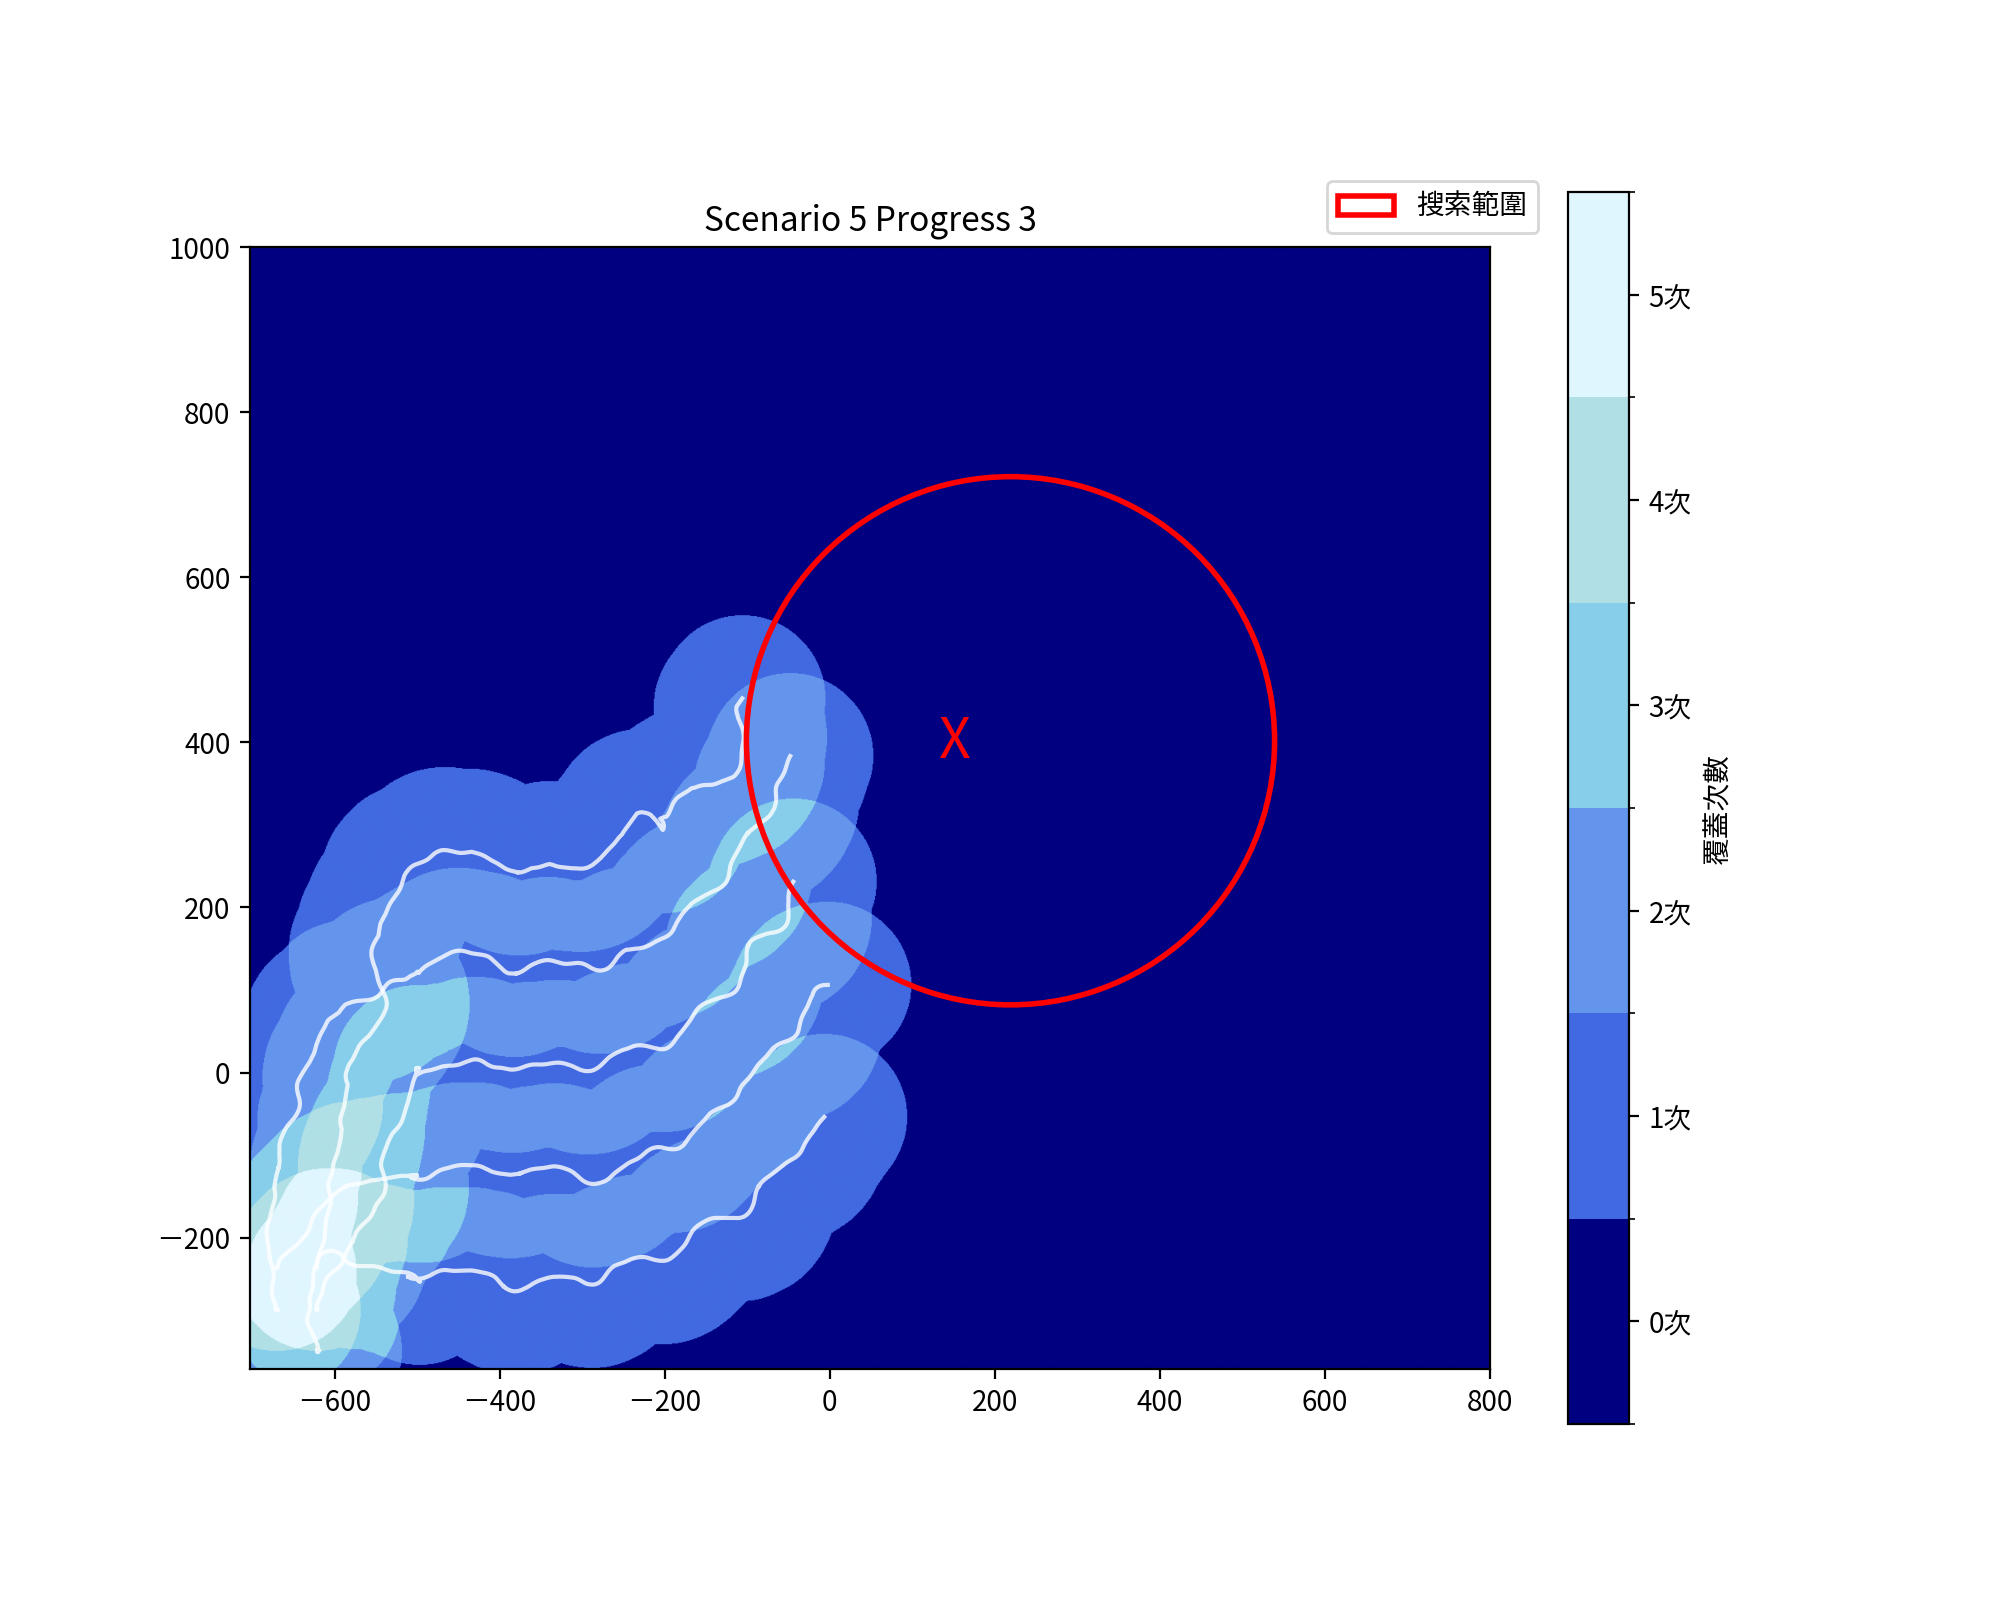
\includegraphics[width=\textwidth]{image/Single3.png}
        \caption{搜尋進度三}
    \end{minipage}
    \hfill
    \begin{minipage}[t]{0.45\textwidth}
        \centering
        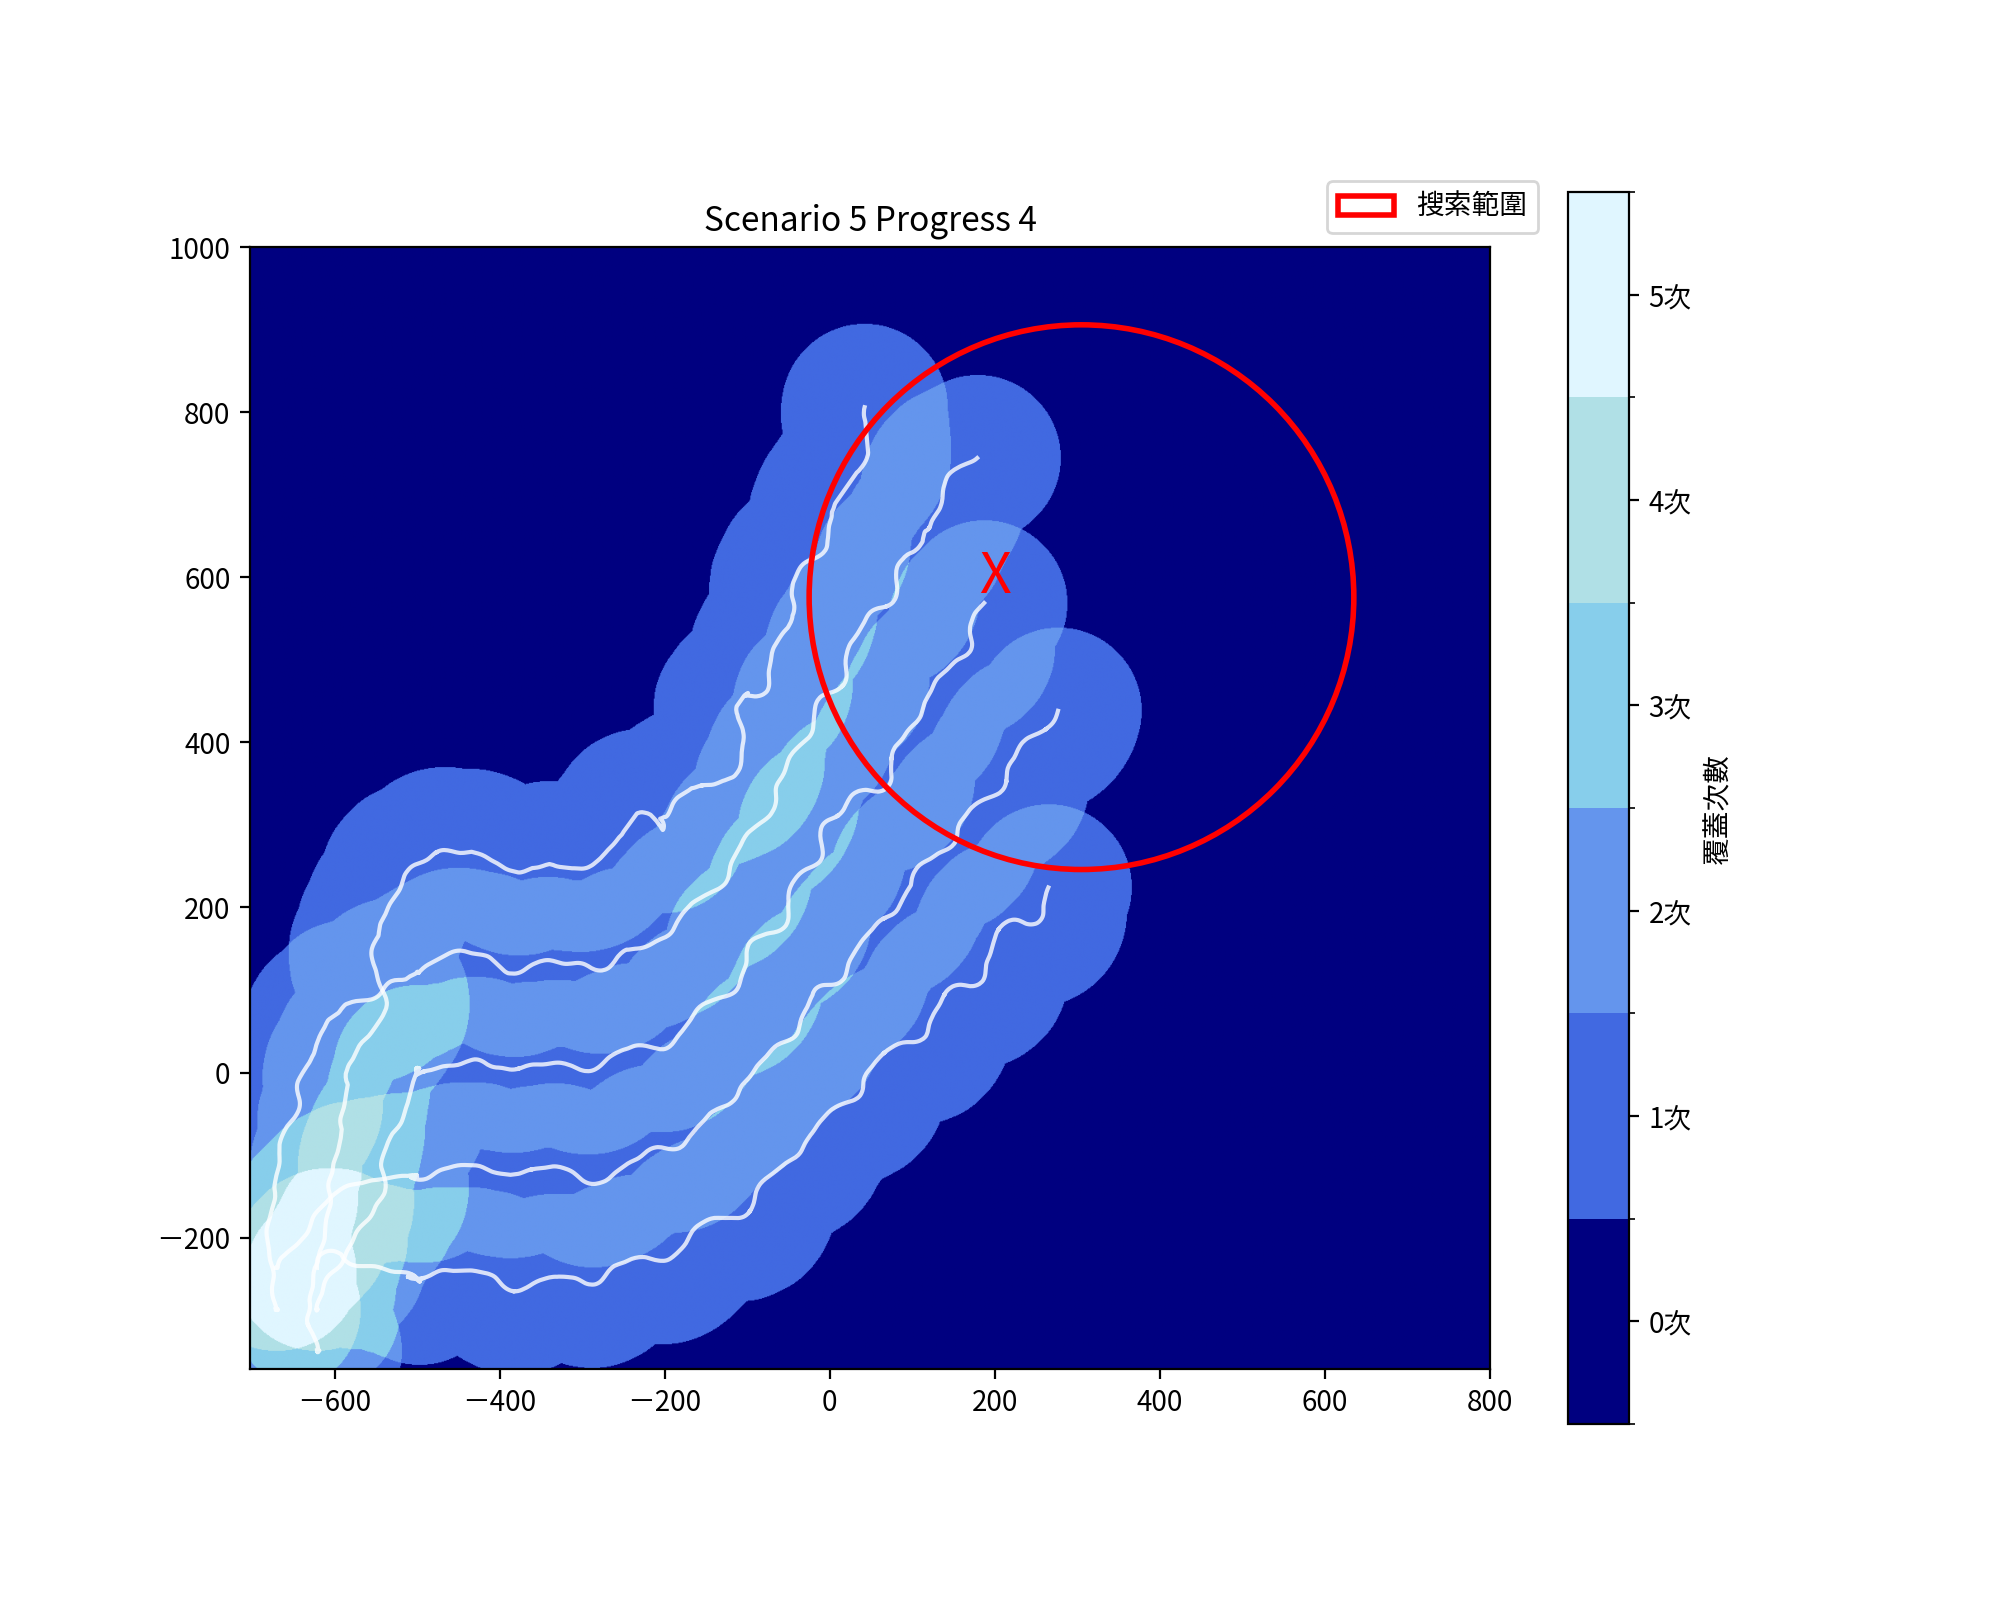
\includegraphics[width=\textwidth]{image/Single4.png}
        \caption{搜尋進度四}
    \end{minipage}
\end{figure}


我們一共進行了 359 次測試,其中 295  次成功,64  次失敗,整體救援率高達 82\%。由於所有船隻都有辦法根據目前紅圈的位置,合理安排搜尋範圍,盡可能涵蓋整個紅圈範圍,而最終的數據顯示,系統一共成功預測 291 次,預測成功率高達 82\%。此結果顯示,我們設計的系統確實能夠在廣闊且情況未知的海域中,以相對低廉的成本的執行平行化搜尋,並有效定位落水者。雖然存在一定比例的失敗案例,但比例有限,且整體數據充分證明系統在本情境中的可行性。

\newpage

\subsubsection{大範圍隨機搜尋任務}

以下兩張圖片是大範圍搜尋任務的執行情況,圖片中的方框為落海者的可能範圍,紅點為實際遇難者的位置,而不同的顏色則代表在搜尋過程中各個位置被不同船隻的搜尋範圍所搜尋的次數,船隊由圖片左下角出發,進入紅框開始搜尋。

\begin{figure}[h]
    \centering
    \begin{minipage}[t]{0.5\textwidth}
        \centering
        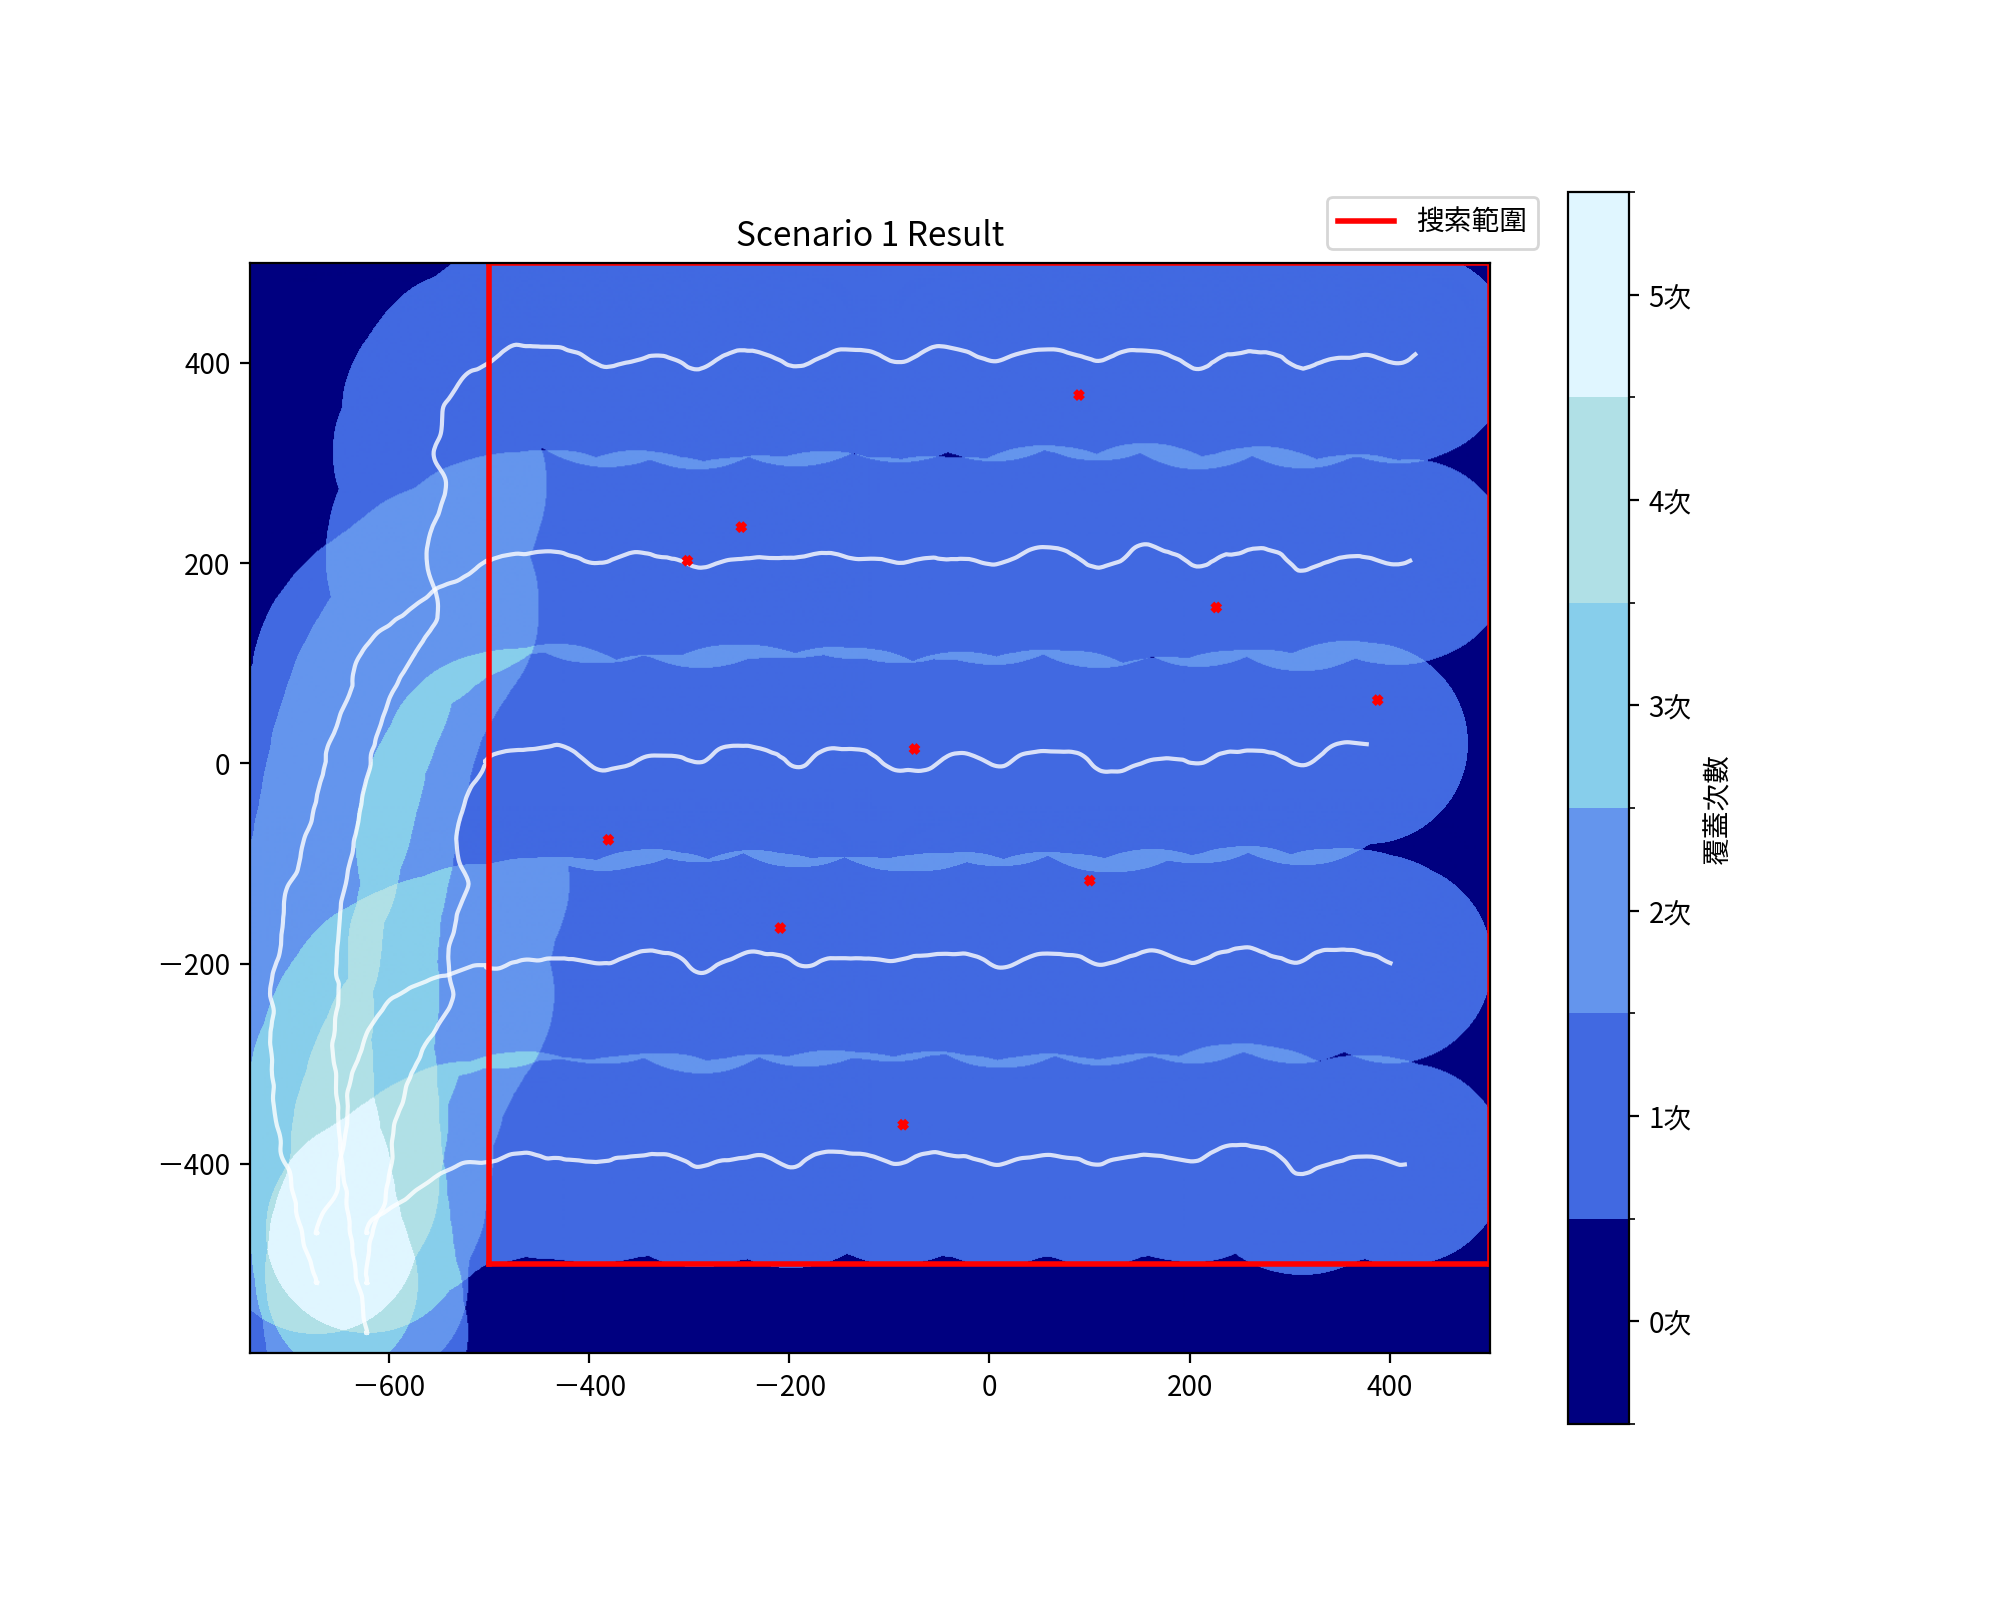
\includegraphics[width=\textwidth]{image/MultiLooseSuccess.png}
        \caption{分散搜尋成功案例}
    \end{minipage}%
    \hfill
    \begin{minipage}[t]{0.5\textwidth}
        \centering
        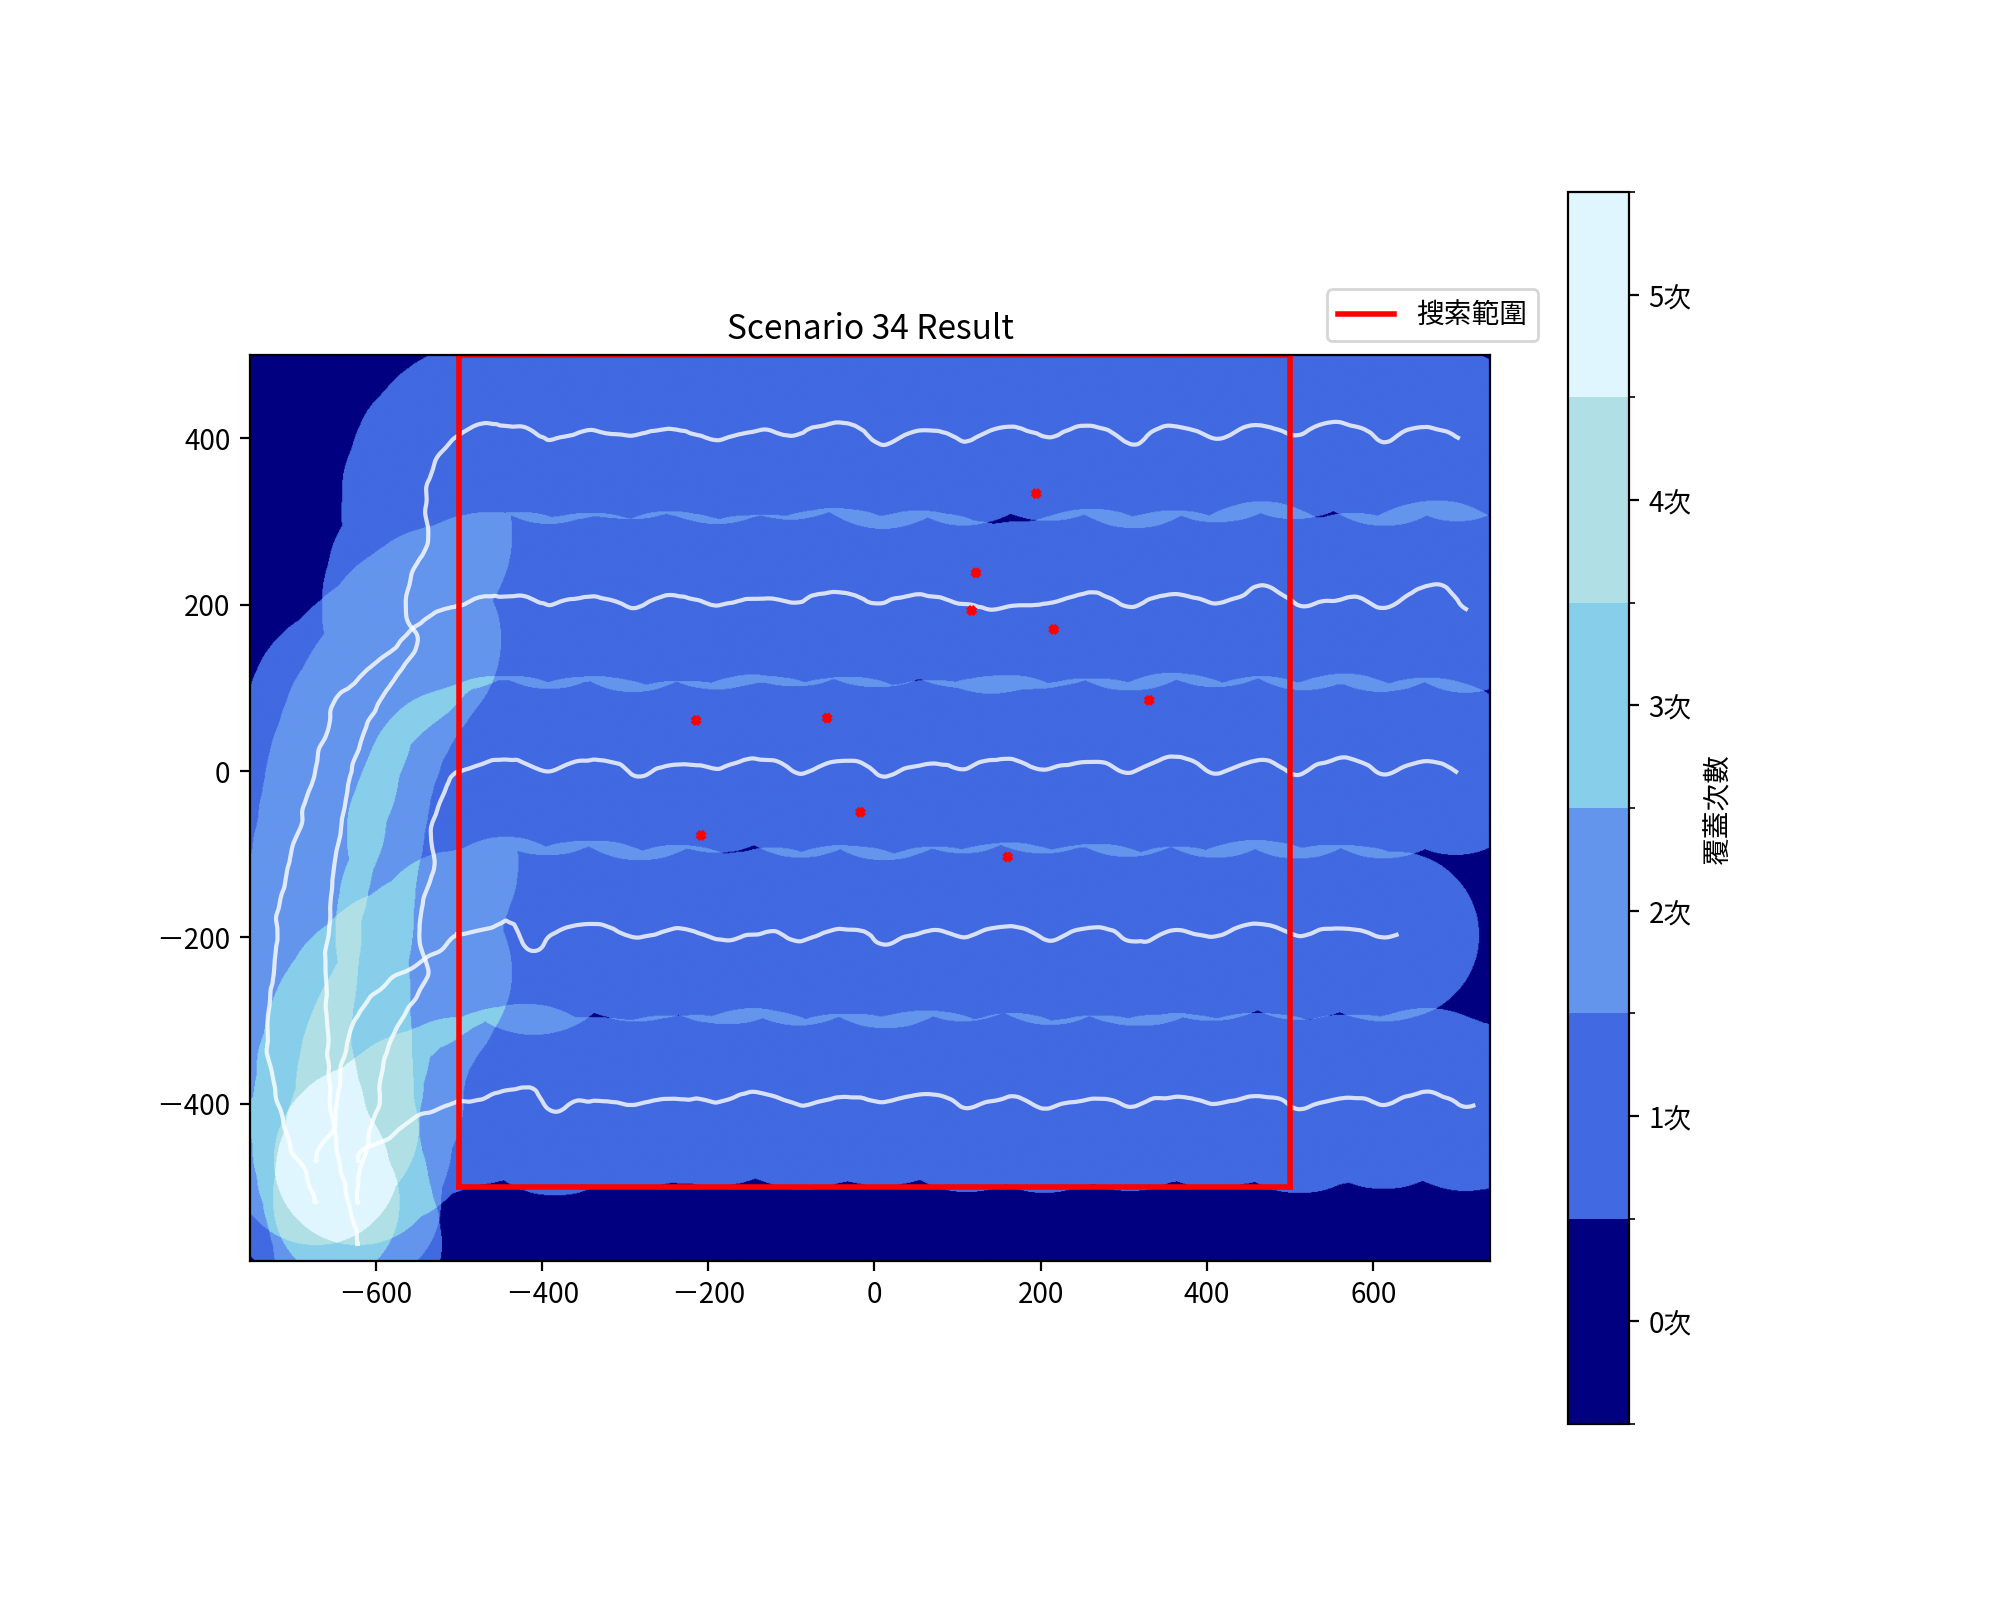
\includegraphics[width=\textwidth]{image/MultiTightSuccess.png}
        \caption{緊密搜尋成功案例}
    \end{minipage}%
\end{figure}

我們一共進行了 109 次測試,在這幾輪測試中,總計模擬了 1070 位落海人士,而系統成功救起了 831 人,整體救援率高達 78\%。此情境主要模擬大型船難、空難海面迫降等大規模搜救任務,在這種情況下,落水人員往往散落在海面各處,傳統的人力搜尋難以快速且全面的掌握其位置。而我們的系統能有效定位分布於不同區域的人員,並將人員位置標示出來,方便救援人員到達現場進行救援。而實驗的結果顯示,我們所設計的自主船舶群集得以在大範圍、高度不確定性的環境中展現不錯的搜尋與定位能力,表現了本系統在大規模災難現場中做為輔助搜救工具的應用潛力。

\newpage

\section{結論與未來發展}

\subsection{研究總結}
本專題針對「海上搜救」所面臨的廣域範圍、高不確定性等挑戰,提出並實作一套「智慧化船舶群集搜救規劃系統」。核心成果如下:
\begin{itemize}
	\item \textbf{建立擬真測試平台}:本專案以 Unity 為主要的開發環境,並結合 Crest 海洋模擬套件,模擬真實風浪與海象。這個組合能夠支援大範圍的海洋場景,並兼顧視覺化與即時模擬的效能,非常適合用於實現海上搜救場景的模擬。
	\item \textbf{開發自主搜救船隻}:使用 ML-Agents 與 DQN 演算法訓練出具備自主導航、避障能力的搜救船隻。
	\item \textbf{設計群集協同策略}:針對多艘船舶進行協同搜尋與任務分配,提升搜救效率。
	\item \textbf{驗證可行性}:透過模擬測試驗證系統在不同搜救場景下的可行性。
\end{itemize}

\subsection{專題成果與限制}
\subsubsection{專題成果}
\paragraph{系統面成果} 本系統能應對單一落水事件及大範圍隨機落水的情境,並且可以根據風向及海流改變搜尋軌跡,進而搜尋到目標

\paragraph{實驗或應用面成果} 單一落水快速救援的環境中,在系統的加持下救援成功率高達 82\%,並且成功預測了 81\% 的人員位置,相較於傳統人工搜救 50\% 的成功率,具有明顯的優勢。

\paragraph{理論或方法面成果} 本研究在演算法與方法上,實現了基於環境感知的導航與避障策略,使船隊能在動態海域環境中自主調整路徑,避免碰撞並保持最佳搜尋覆蓋率。

\paragraph{應用與價值} 本系統具備在大型船難、空難迫降或軍事與民用搜救等情境下的應用潛能。其低成本、高效率的搜尋方式,能減少人力依賴並提升救援成功率,對於提升整體搜救資源運用效率具有重要價值。未來若能結合真實感測數據與更複雜的環境建模,將有助於推動自主搜救技術在實務上的落地與推廣。

\subsubsection{研究限制}
\paragraph{實驗設計限制} 由於本研究主要在模擬環境中進行,無法涵蓋真實海域中可能出現的各種不確定性,例如:雷擊等特殊情況。實驗中所設定的參數僅能代表部分典型情境,因此結果雖具參考價值,但仍需進一步實地驗證。  

\paragraph{方法論限制} 在嘗試多代理訓練時,由於環境複雜或演算法設計限制,訓練過程往往難以收斂且穩定性較低。因此本研究採用單代理訓練方式,雖能在系統統籌下有效完成多代理搜尋任務,但因此缺少多代理協作所帶來的潛在優勢。這也是未來研究需要進一步探討的方向。


\paragraph{時間與資源限制}  受限於研究時間與資源,本研究無法取得實際的船舶設備或海上場域進行驗證,相關實驗僅止於模擬層面。

\subsection{未來研究方向}
\paragraph{多代理協作訓練}  引入多代理強化學習或協作演算法,提升船隊在複雜環境下的協作效率與搜尋成功率。針對多代理訓練難以收斂的問題,可探索分層控制、經驗共享或穩定化策略,改善訓練穩定性。

\paragraph{更真實的環境} 優化模擬環境並加入更多變因,提升系統的真實性。

\paragraph{更多搜尋策略} 加入更多搜尋策略,讓系統可以適應不同規模的任務性質及搜救任務,增加系統的應用範圍。

\paragraph{連接到實體測試} 將系統應用在實際的水面上,結合實時風向、海流及各種感測數據進行搜救測試,驗證其可靠性。

\subsection{可行的解決方案}
\paragraph{多代理協作改進} 採用分層控制或經驗共享策略進行多代理訓練,可減少訓練不收斂的風險,提升船隊在動態環境下的協作效率。透過模擬不同海域與任務規模,逐步調整協作演算法,達成穩定且可擴展的多代理系統。

\paragraph{環境模擬精度提升}  
引入更精細的海流、風向以及潮汐資料,改善模擬精度,使系統在不同環境變化下能更準確地預測落水者位置。可使用歷史數據或即時資料進行校正,縮小模擬與現實的差距。

\newpage

\begin{thebibliography}{9}
\bibitem{KilicChallenge}
Kilic, K. I., Maity, S., Sung, I., \& Nielsen, P. (2025). 
Challenges and AI-Driven Solutions in Maritime Search and Rescue Planning: A Comprehensive Literature Review. 
Marine Policy, 178, Article 106692. 
\url{https://doi.org/10.1016/j.marpol.2025.106692}

\bibitem{KilicRL}
Kilic, K. I., Maity, S., Sung, I., \& Nielsen, P. (2025). 
A Reinforcement Learning-Assisted Search and Rescue Resource Allocation Decision-Making Approach for Maritime Emergencies. 
Computers \& Industrial Engineering, 201, Article 110933. 
\url{https://doi.org/10.1016/j.cie.2025.110933}

\bibitem{GroupMobile}
Yang, T., Jiang, Z., Sun, R., Cheng, N., \& Feng, H. (2020). 
Maritime Search and Rescue Based on Group Mobile Computing for Unmanned Aerial Vehicles and Unmanned Surface Vehicles. 
IEEE Transactions on Industrial Informatics, 16(12), 7700-7708. 
\url{https://doi.org/10.1109/TII.2020.2974047}

\bibitem{USCoastGuard}
U.S. Department of Homeland Security United States Coast Guard. (2013). 
U.S. Coast Guard Addendum to the United States National Search and Rescue Supplement (NSS) to the International Aeronautical and Maritime Search and Rescue Manual (IAMSAR).

\bibitem{NOAA}
Search and Rescue. (n.d.). 
NOAA-National Oceanic and Atmospheric Administration. 
\url{https://www.sarsat.noaa.gov/search-and-rescue/}

\bibitem{Survey}
Li, J., Zhang, G., Jiang, C., \& Zhang, W. (2023). 
A Survey of Maritime Unmanned Search System: Theory, Applications and Future Directions. 
Ocean Engineering, 285(1), Article 115359. 
\url{https://doi.org/10.1016/j.oceaneng.2023.115359}

\bibitem{IAMSAR2008}
IMO, \& ICAO. (2008). 
IAMSAR Manual Volume II: Mission Co-Ordination 2008 Edition.

\bibitem{IAMSAR2016}
IMO, \& ICAO. (2016). 
IAMSAR Manual Volume III: Mobile Facilities 2016 Edition.

\bibitem{Oways}
Oways. (2024). 
IAMSAR Search Patterns Explained with Sketches - Oways Online. 
\url{https://owaysonline.com/iamsar-search-patterns/}

\bibitem{MLAgentRepo}
Maryamziaa. (n.d.). 
ml-agents [GitHub Repository]. 
GitHub. 
\url{https://github.com/Unity-Technologies/ml-agents}

\bibitem{CrestIntro}
Introduction. (n.d.). 
Crest Ocean System. 
\url{https://crest.readthedocs.io/en/stable/about/introduction.html}

\bibitem{AiCoverage}
Ai, B., Jia, M., Xu, H., Xu, J., Wen, Z., Li, B., \& Zhang, D. (2021). 
Coverage Path Planning for Maritime Search and Rescue Using Reinforcement Learning. 
Ocean Engineering, 241, Article 110098.
\url{https://doi.org/10.1016/j.oceaneng.2021.110098}

\bibitem{PathPlanning}
Zhang, A., Wang, W., Bi, W., \& Huang, Z. (2024). 
A Path Planning Method Based on Deep Reinforcement Learning for AUV in Complex Marine Environment. 
Ocean Engineering, 313(1), Article 119354. 
\url{https://doi.org/10.1016/j.oceaneng.2024.119354}

\bibitem{EnhancedPathPlanning}
Zhangahmad, J., \& Wahab, M. N. (2025). 
Enhancing the Safety and Smoothness of Path Planning through an Integration of Dijkstra's Algorithm and Piecewise Cubic Bezier Optimization. 
Expert Systems with Applications, 289(15), Article 128315. 
\url{https://doi.org/10.1016/j.eswa.2025.128315}

\bibitem{SimulationHeuristic}
Ugwoke, K. C., Nnanna, N. A., \& Abdullahi, S. E. (2025). 
Simulation-based review of classical, heuristic, and metaheuristic path planning algorithms. 
Scientific Reports, 15, 12643. 
\url{https://doi.org/10.1038/s41598-025-96614-2}

\bibitem{Ennong}
Ennong, T., Ye, L., Teng, M., Yulei, L., Yueming, L., \& Jian, C. (2024). 
Design and Experiment of a Sea-Air Heterogeneous Unmanned Collaborative System for Rapid Inspection Tasks at Sea. 
Applied Ocean Research, 143, Article 103856. 
\url{https://doi.org/10.1016/j.apor.2023.103856}

\bibitem{Rolls}
熊治民. (2018). 
自主航行船舶(無人船)發展趨勢. 
經濟部產業技術司. 
\url{https://www.moea.gov.tw/MNS/doit/industrytech/IndustryTech.aspx?menu_id=13545&it_id=202}

\bibitem{Hyundai}
周家仰. (2023). 
韓造船業者無人船建造較原設定目標提前6年. 
航貿周刊. 
\url{https://shippingdigest.tw/news/20230605n1}

\bibitem{autoboat}
李孟諺. (2022). 
離岸風場運維無人船應用趨勢探討. 
經濟部產業技術司. 
\url{https://www.moea.gov.tw/MNS/doit/industrytech/IndustryTech.aspx?menu_id=13545&it_id=444}

\bibitem{Yara}
Yara Birkeland, Two Years On. (2024). 
Yara | Leader in Crop Nutrition, Ammonia and Industrial Solutions. 
\url{https://www.yara.com/knowledge-grows/yara-birkeland-two-years-on/}

\bibitem{Meguri}
The Nippon Foundation MEGURI2040 Fully Autonomous Ship Program. (n.d.). 
The Nippon Foundation. 
\url{https://en.nippon-foundation.or.jp/what/projects/ocean/meguri204}

\bibitem{DiffAgent}
How Do Multi-Agent Systems Differ from Single-Agent Systems? (n.d.). 
Milvus. 
\url{https://milvus.io/ai-quick-reference/how-do-multiagent-systems-differ-from-singleagent-systems}

\bibitem{MultiAgent}
Gutowska, A. (n.d.). 
What Is a Multi-Agent System? 
IBM. 
\url{https://www.ibm.com/think/topics/multiagent-system}

\bibitem{MultiChallenge}
Canese, L., Cardarilli, G. C., Di Nunzio, L., Fazzolari, R., Giardino, D., Re, M., \& Spanò, S. (2021). 
Multi-Agent Reinforcement Learning: A Review of Challenges and Applications. 
Applied Sciences, 11(11), 4948. 
\url{https://doi.org/10.3390/app11114948}

\bibitem{DQN}
Zhang, H., Bai, F., Xiao, C., Gao, C., Xu, B., \& Müller, M. (2025). 
β-DQN: Improving Deep Q-Learning By Evolving the Behavior. 
Proceedings of the 24th International Conference on Autonomous Agents and Multiagent Systems (AAMAS 2025), IFAAMAS, 2317-2319. 
\url{https://dl.acm.org/doi/10.5555/3709347.3743872}

\bibitem{DRL2018}
李宏毅. (n.d.). 
Book\_李宏毅老師Deep Reinforcement Learning 2018課程筆記. 
HackMD. 
\url{https://hackmd.io/@shaoeChen/Bywb8YLKS/https\%3A\%2F\%2Fhackmd.io\%2F\%40shaoeChen\%2FHkH2hSKuS}

\bibitem{DRLAutonomous}
Zhang, M., et al. (2024). 
Deep Reinforcement Learning in Autonomous Car Path Planning and Control: A Survey. 
arXiv preprint arXiv:2404.00340v1.

\bibitem{DRLBased}
Chen, L., Jiang, Z., Cheng, L., Knoll, A. C., \& Zhou, M. (2022). 
Deep Reinforcement Learning Based Trajectory Planning Under Uncertain Constraints. 
Frontiers in Neurorobotics, 16. 
\url{https://doi.org/10.3389/fnbot.2022.883562}

\bibitem{PathPlanningMethod}
Zhang, A., Wang, W., Bi, W., \& Huang, Z. (2024). 
A Path Planning Method Based on Deep Reinforcement Learning for AUV in Complex Marine Environment. 
Ocean Engineering, 313(1), Article 119354. 
\url{https://doi.org/10.1016/j.oceaneng.2024.119354}

\bibitem{Atari}
Mnih, V., Kavukcuoglu, K., Silver, D., Graves, A., Antonoglou, I., Wierstra, D., \& Riedmiller, M. (2013). 
Playing Atari with deep reinforcement learning. 
arXiv. 
\url{https://doi.org/10.48550/arXiv.1312.5602}

\bibitem{SAC}
晴晴\_amanda. (2020). 
RL策略梯度方法之(十四):Soft Actor-Critic (SAC). 
CSDN. 
\url{https://blog.csdn.net/qq_38293297/article/details/108919306}

\bibitem{rybchak2024}
Rybchak, Z., \& Kopylets, M. (2024). 
Comparative Analysis of DQN and PPO Algorithms in UAV Obstacle Avoidance 2D Simulation. 
CEUR Workshop Proceedings, 3688, 391-403. 
\url{https://ceur-ws.org/Vol-3688/paper25.pdf}

\bibitem{greenberg}
Greenberg, V., \& Hernandez, C. (2024). 
Autonomous Drone Navigation for First Response (CS224R final project report). 
Stanford University. 
\url{https://cs224r.stanford.edu/projects/pdfs/CS224r__report.pdf}

\bibitem{Drew2021}
Drew, D. S. (2021). 
Multi-Agent Systems for Search and Rescue Applications. 
Current Robotics Reports, 2, 189-200. 
\url{https://doi.org/10.1007/s43154-021-00048-3}

\bibitem{Ericyangyu}
Ericyangyu. (n.d.). 
PPO-for-Beginners [GitHub Repository]. 
GitHub. 
\url{https://github.com/ericyangyu/PPO-for-Beginners}

\bibitem{Idrees}
Hossain, J. (n.d.). 
Autonomous Driving with Deep Reinforcement Learning in CARLA Simulation. 
arXiv. 
\url{https://doi.org/10.48550/arXiv.2306.11217}

\bibitem{TimeLimits2017}
Pardo, F., Tavakoli, A., Levdik, V., \& Kormushev, P. (2018). 
Time Limits in Reinforcement Learning. 
Proceedings of the 35th International Conference on Machine Learning (ICML 2018), 80, 4045-4054. 
\url{https://doi.org/10.48550/arXiv.2306.11217}

\end{thebibliography}

\end{document}